\documentclass[preprint]{imsart}
%\documentclass[bj]{imsart}

\usepackage{lineno,hyperref}


\usepackage{aliascnt}
\usepackage{amsmath}
\usepackage{amssymb}
\usepackage{amsthm}
\usepackage{bibentry}
\usepackage{bbm}
\usepackage{booktabs}
\usepackage{color}
\usepackage{enumerate}
\usepackage{float}
\usepackage{graphicx}
\usepackage{hyperref}
\usepackage{ifthen}
\usepackage{mathtools}
\usepackage[numbers]{natbib}
\usepackage[linesnumbered,vlined]{algorithm2e}
\usepackage{stmaryrd}
\usepackage{ushort}
\usepackage{xargs}


\RequirePackage[colorlinks,citecolor=blue,urlcolor=blue]{hyperref}

% provide arXiv number if available:
%\arxiv{arXiv:0000.0000}

% put your definitions there:
\startlocaldefs


%\providecommand*{\definitionautorefname}{Definition}
%\providecommand*{\lemmaautorefname}{Lemma}
%\providecommand*{\exampleautorefname}{Example}
\providecommand*{\propositionautorefname}{Proposition}
%\providecommand*{\exerciseautorefname}{Exercise}
%\providecommand*{\corollaryautorefname}{Corollary}
%\providecommand*{\chapterautorefname}{Chapter}
%\providecommand*{\partautorefname}{Part}
%\providecommand*{\remarkautorefname}{Remark}
%\renewcommand*\sectionautorefname{Section} 
%
%
%
\newtheorem{theorem}{Theorem}
\newaliascnt{proposition}{theorem}
\newtheorem{proposition}[proposition]{Proposition}
\aliascntresetthe{proposition}
%
\newaliascnt{lemma}{theorem}
\newtheorem{lemma}[lemma]{Lemma}
\aliascntresetthe{lemma}
%
%\newaliascnt{corollary}{theorem}
%\newtheorem{corollary}[corollary]{Corollary}
%\aliascntresetthe{corollary}
%
\newaliascnt{definition}{theorem}
\newtheorem{definition}[definition]{Definition}
\aliascntresetthe{definition}
%
\newaliascnt{example}{theorem}
\newtheorem{example}[example]{Example}
\aliascntresetthe{example}
%
\newaliascnt{remark}{theorem}
\newtheorem{remark}[remark]{Remark}
\aliascntresetthe{remark}

% A

\newcommandx\A[2][1=]{
\ifthenelse{\equal{#1}{}}
{\hspace{-1mm}(\textbf{A\ref{#2}})\hspace{-1mm}}
{\hspace{-1mm}(\textbf{A\ref{#1}--\ref{#2}})\hspace{-1mm}}
}

% B

\newcommandx\B[2][1=]{
\ifthenelse{\equal{#1}{}}
{\hspace{-1mm}(\textbf{S})\hspace{-1mm}}
{\hspace{-1mm}(\textbf{S\ref{#1}--\ref{#2}})\hspace{-1mm}}
}
%\newcommandx\B[2][1=]{
%\ifthenelse{\equal{#1}{}}
%{\hspace{-1mm}(\textbf{S\ref{#2}})\hspace{-1mm}}
%{\hspace{-1mm}(\textbf{S\ref{#1}--\ref{#2}})\hspace{-1mm}}
%}
\newcommand{\bd}{c}
\newcommand{\bias}[2]{\beta_{#2} \langle #1 \rangle} 
\newcommand{\biasfilt}[2]{\bar{\beta}_{#2} \langle #1 \rangle} 
\newcommand{\binset}[1]{\mathsf{I}_{#1}}
\newcommand{\Binsp}[1]{\mathsf{B}_{#1}}
\newcommand{\bmf}[1]{\mathbb{F}(#1)}


% C

\newcommand{\cat}{\mathsf{Cat}}
\newcommand{\chunk}[3]{{#1}_{#2}^{#3}}

% D 

\newcommand{\DDelta}[3]{\Delta_{#1}\langle #2\rangle(#3)}
\newcommand{\dlim}{\stackrel{\mathcal D}{\longrightarrow}}

% E

\newcommand{\E}{\mathbb{E}}
\newcommand{\ed}{g}
\newcommand{\Efd}{\mathcal{E}}
\newcommand{\enoch}[3]{E_{#1,#2}^{#3}}
\newcommand{\epart}[2]{\xi_{#1}^{#2}}
\newcommand{\eqdef}{\vcentcolon=}
\newcommand{\Esp}{\mathsf{E}}
\newcommandx{\eve}[3][1=]{\ifthenelse{\equal{#1}{}}{E_{#2}^{#3}}{E_{#1,#2}^{#3}}}

% F

\newcommandx{\filt}[1][1=]{\ifthenelse{\equal{#1}{}}{\filtsymb}{\filtsymb \langle #1 \rangle}}
\newcommand{\filtpart}[1][1=]{\ifthenelse{\equal{#1}{}}{\filtsymb_\N}{\filtsymb_\N \langle #1 \rangle}}
\newcommand{\filtsymb}{\bar{\eta}}
\newcommandx{\filtvariance}[3][1=,3=]{\bar{\sigma}^{#1}_{#3} \langle #2 \rangle}

% G

\newcommandx{\gen}[1][1=]{\ifthenelse{\equal{#1}{1}}{G}{G'}} 
\newcommand{\genkernel}{\kernel{K}}

% H

\newcommand{\hk}{\kernel{M}}


% I

\newcommand{\init}{\chi}
\newcommand{\ind}[2]{I_{#1}^{#2}}
\newcommand{\intvect}[2]{\llbracket #1, #2 \rrbracket}

% K 

\newcommand{\kernel}[1]{\mathbf{#1}}

% L

\newcommand{\lag}{\lambda}
\newcommand{\lagtime}[2]{#1(#2)}
%\newcommand{\lagtime}[2]{\langle #1 \rangle_{#2}}
\newcommandx{\likeli}[3][1=]{\pi_{#1} \langle #2 \rangle(#3)}
\newcommand{\limitfunc}[1]{\pi \langle #1 \rangle}

% M

\newcommand{\md}{m}
\newcommand{\mdlow}{\ushort{\varepsilon}}
\newcommand{\mdup}{\bar{\varepsilon}}
%\newcommand{\mdr}{\mathcal{M}}
\newcommand{\mdr}{\mathbb{M}}
\newcommand{\me}{\mathrm{e}}
\newcommand{\mk}{\kernel{M}}
\newcommand{\mklow}{\ushort{\varepsilon}}
\newcommand{\mkup}{\bar{\varepsilon}}
\newcommand{\mumeas}[2]{\mu_{#1} \langle #2 \rangle}

% N

\newcommand{\N}{N}
\newcommand{\nset}{\mathbb{N}}
\newcommand{\nsetpos}{\mathbb{N}^\ast}

% O

\newcommand{\1}{\mathbbm{1}}
\newcommand{\ordo}{\mathcal{O}}

% P 

\newcommand{\p}{p}
\newcommand{\partfd}[1]{\mathcal{F}_{#1}}
\newcommand{\per}{\zeta}
\newcommand{\perblock}{\bar{\zeta}}
\newcommand{\plim}{\stackrel{\prob}{\longrightarrow}}
\newcommandx{\pot}[1][1=]{\ifthenelse{\equal{#1}{}}{g}{g \langle #1 \rangle}}
\newcommand{\potlow}{\ushort{\delta}}
\newcommand{\potup}{\bar{\delta}}
\newcommand{\predsymb}{\eta}
\newcommandx{\pred}[1][1=]{\ifthenelse{\equal{#1}{}}{\predsymb}{\predsymb \langle #1 \rangle}}
\newcommand{\predpart}[1][1=]{\ifthenelse{\equal{#1}{}}{\predsymb_\N}{\predsymb_\N \langle #1 \rangle}}
\newcommand{\prob}{\mathbb{P}}
\newcommand{\probmeas}[1]{\mathbb{M}(#1)}
\newcommand{\probdoeblin}[2]{\mu_{#1} \langle #2 \rangle}
\newcommand{\rmd}{\mathrm{d}}

% R

\newcommand{\rate}{\rho}
\newcommand{\refm}{\nu}
\newcommand{\rset}{\mathbb{R}}
\newcommand{\rsetpos}{\mathbb{R}^\ast_+}

% S

% T

\newcommand{\tbw}{\emph{(To be written.)}}
\newcommand{\term}[3][]{\upsilon_{#2,#3} \langle #1 \rangle}
%\newcommand{\thickhline}{%
%    \noalign {\ifnum 0=`}\fi \hrule height 2pt
%    \futurelet \reserved@a \@xhline
%}
%\newcolumntype{w}{@{\hskip\tabcolsep\vrule width 2pt\hskip\tabcolsep}}
%\makeatother

% U 

\newcommandx{\uk}[1][1=]{\ifthenelse{\equal{#1}{}}{\kernel{Q}}{\kernel{Q} \langle #1 \rangle}}
\newcommand{\unitstr}[2]{1_{#1}}
\newcommand{\unpredsymbol}{\gamma}
\newcommandx{\unpred}[1][1=]{\ifthenelse{\equal{#1}{}}{\unpredsymb}{\unpredsymb \langle #1 \rangle}}
\newcommand{\unpredpart}[1][1=]{\ifthenelse{\equal{#1}{}}{\unpredsymbol_\N}{\unpredsymbol_\N \langle #1 \rangle}}

% V 

\newcommandx{\varest}[3][1=,3=]{\ifthenelse{\equal{#3}{}}{\sigma^{#1}_\N \langle #2 \rangle}{\sigma^{#1}_{\N, #3} \langle #2 \rangle}}
\newcommandx{\varestfilt}[3][1=,3=]{\ifthenelse{\equal{#3}{}}{\bar{\sigma}^{#1}_\N \langle #2 \rangle}{\bar{\sigma}^{#1}_{\N, #3} \langle #2 \rangle}}
\newcommandx{\variance}[3][1=,3=]{\sigma^{#1}_{#3} \langle #2 \rangle}


% W 

\newcommand{\wgt}[2]{\omega_{#1}^{#2}}
\newcommand{\wgtsum}[1]{\Omega_{#1}}

% X 

\newcommand{\Xsp}{\mathsf{X}}
\newcommand{\Xfd}{\mathcal{X}}

% Y

\newcommand{\Ysp}{\mathsf{Y}}
\newcommand{\Yfd}{\mathcal{Y}}

% Z

\newcommand{\zerostr}[1]{0_{#1}}
\newcommand{\Zsp}{\mathsf{Z}}
\newcommand{\Zfd}{\mathcal{Z}}
\newcommand{\zset}{\mathbb{Z}}

% Hypotheses

\newcounter{hypA}
\newenvironment{hypA}{\refstepcounter{hypA}\begin{itemize}
  \item[({\bf A\arabic{hypA}})]}{\end{itemize}}
%\newenvironment{hypA}{\begin{sf}\refstepcounter{hypA}\begin{itemize}
%  \item[({\bf A\arabic{hypA}})]}{\end{itemize}\end{sf}}

\newcounter{hypB}
%\newenvironment{hypB}{\refstepcounter{hypB}\begin{itemize}
%  \item[({\bf S\arabic{hypB}})]}{\end{itemize}}
\newenvironment{hypB}{\refstepcounter{hypB}\begin{itemize}
  \item[({\bf S})]}{\end{itemize}}



\endlocaldefs

\begin{document}

\begin{frontmatter}

% "Title of the Paper"

\title{Numerically stable online estimation of variance in particle filters}

\runtitle{Estimation of variance in particle filters}

\begin{aug}
\author{\fnms{Jimmy} \snm{Olsson}\thanksref{a,t1}\ead[label=e1]{jimmyol@kth.se}}
\and
\author{\fnms{Randal} \snm{Douc}\thanksref{b}\ead[label=e2]{randal.douc@it-sudparis.eu}}

\address[a]{Department of Mathematics \\
KTH Royal Institute of Technology \\
SE-100 44  Stockholm, Sweden \\
\printead{e1}}

\address[b]{D\'epartement CITI \\ 
TELECOM SudParis \\
9 rue Charles Fourier, 91000 EVRY \\
\printead{e2}}

\thankstext{t1}{J.~Olsson is supported by the Swedish Research Council, Grant 2011-5577.}

\runauthor{J. Olsson and R. Douc}

\affiliation{KTH Royal Institute of Technology and Institut T\'el\'ecom/T\'el\'ecom SudParis}

\end{aug}

\begin{abstract}
\begin{abstract}
%Although Deep Convolutional Neural Networks (CNNs) have liberated their power in various computer vision tasks, the most important components of CNN, convolutional layers and fully connected layers, are still limited to linear transformations. In this paper, we propose a novel Factorized Bilinear (FB) layer to model the pairwise feature interactions by considering the quadratic terms in the transformations. Compared with existing methods that tried to incorporate complex non-linearity structures into CNNs, the factorized parameterization makes our FB layer only require a linear increase of parameters and affordable computational cost. To further reduce the risk of overfitting of the FB layer, a specific remedy called DropFactor is devised during the training process. We also analyze the connection between FB layer and some existing models, and show FB layer is a generalization to them. Finally, we validate the effectiveness of FB layer on several widely adopted datasets including CIFAR-10, CIFAR-100 and ImageNet, and demonstrate superior results compared with various state-of-the-art deep models.

Neural Style Transfer~\cite{neuralart} has recently demonstrated very exciting results which catches eyes in both academia and industry. Despite the amazing results, the principle of neural style transfer, especially why the Gram matrices could represent style remains unclear. In this paper, we propose a novel interpretation of neural style transfer by treating it as a domain adaptation problem. Specifically, we theoretically show that matching the Gram matrices of feature maps is equivalent to minimize the Maximum Mean Discrepancy (MMD) with the second order polynomial kernel. Thus, we argue that the essence of neural style transfer is to match the feature distributions between the style images and the generated images. To further support our standpoint, we experiment with several other distribution alignment methods, and achieve appealing results. We believe this novel interpretation connects these two important research fields, and could enlighten future researches.

\end{abstract}
\end{abstract}

\begin{keyword}[class=MSC]
\kwd[Primary ]{62M09}
%\kwd{}
\kwd[; secondary ]{62F12}
\end{keyword}


\begin{keyword}
\kwd{Asymptotic variance}
\kwd{Feynman-Kac models}
\kwd{hidden Markov models}
\kwd{particle filters}
\kwd{sequential Monte Carlo methods}
\kwd{state-space models}
\kwd{variance estimation}
\end{keyword}

% history:
% \received{\smonth{1} \syear{0000}}

%\tableofcontents

\end{frontmatter}

% Introduction
\section{Introduction}
\label{sec:introduction}
\begin{section}{Introduction}

Transferring the style from one image to another image is an interesting yet difficult problem. There have been many efforts to develop efficient methods for automatic style transfer~\cite{hertzmann2001image,efros2001image,efros1999texture,shih2014style,kwatra2005texture}. Recently, Gatys \emph{et al.} proposed a seminal work~\cite{neuralart}: It captures the style of artistic images and transfer it to other images using Convolutional Neural Networks (CNN). This work formulated the problem as finding an image that matching both the content and style statistics based on the neural activations of each layer in CNN. It achieved impressive results and several follow-up works improved upon this innovative approaches~\cite{johnson2016perceptual,ulyanov2016texture,ruder2016artistic,ledig2016photo}. Despite the fact that this work has drawn lots of attention, the fundamental element of style representation: the Gram matrix in~\cite{neuralart} is not fully explained. The reason why Gram matrix can represent artistic style still remains a mystery.

In this paper, we propose a novel interpretation of neural style transfer by casting it as a special domain adaptation~\cite{beijbom2012domain,patel2015visual} problem. We theoretically prove that matching the Gram matrices of the neural activations can be seen as minimizing a specific Maximum Mean Discrepancy (MMD)~\cite{mmd}. This reveals that neural style transfer is intrinsically a process of distribution alignment of the neural activations between images. Based on this illuminating analysis, we also experiment with other distribution alignment methods, including MMD with different kernels and a simplified moment matching method. These methods achieve diverse but all reasonable style transfer results. Specifically, a transfer method by MMD with linear kernel achieves comparable visual results yet with a lower complexity. Thus, the second order interaction in Gram matrix is not a must for style transfer. Our interpretation provides a promising direction to design style transfer methods with different visual results. To summarize, our contributions are shown as follows:
\begin{enumerate}
\item First, we demonstrate that matching Gram matrices in neural style transfer~\cite{neuralart} can be reformulated as minimizing  MMD with the second order polynomial kernel.
\item Second, we extend the original neural style transfer with different distribution alignment methods based on our novel interpretation.
\end{enumerate}

\end{section}

% Preliminaries
\section{Preliminaries}
\label{sec:preliminaries}
% !TeX root = main.tex
\section{Preliminaries}


\subsection{CAT(0) cube complexes and pocsets}

We begin by a short survey of definitions concerning CAT(0) cube complexes and pocsets. A reader who is acquainted with the basic terminology can skip this subsection. For further details see, for example, Sageev \cite{Sag12}.

A \emph{cube complex} is a collection of euclidean cubes of various dimensions in which subcubes have been identified isometrically. 

A simplicial complex is \emph{flag} if every $(n+1)$-clique in its 1-skeleton spans a $n$-simplex.
A cube complex is \emph{non-positively curved} (NPC) if the link of every vertex is a flag simplicial complex. It is a \emph{\CCC} if moreover it is simply connected.

A cube complex $\CC{X}$ can be equipped with two natural metrics, the euclidean and the $L^1$-metric. With respect to the former $\CC{X}$ is NPC if and only if it is NPC \`{a} la Gromov (see Gromov \cite{Gro87} or Bridson and Haefliger \cite{BrHa99}). While the latter is more natural to the combinatorial structure of CAT(0) cube complexes described below.

Given a cube $\CCc{C}$ and an edge $\CCc{e}$ of $\CCc{C}$. The midcube of $\CCc{c}$ associated to $\CCc{e}$ is the convex hull of the midpoints of $\CCc{e}$ and the edges parallel to $\CCc{e}$.
A \emph{hyperplane} associated to $\CCc{e}$ is the smallest subset containing the midpoint of $\CCc{e}$ and such that if it contains a midpoint of an edge it contains all the midcubes containing it.
Every hyperplane $\hyp{h}$ in a \CCC $\CC{X}$ separates $\CC{X}$ into exactly two components, see for example Niblo and Reeves \cite{NiRe98}, called the \emph{halfspaces} associated to $\hyp{h}$. A hyperplane can thus also be abstractly viewed as a pair of complementary halfspaces. 
%The \emph{carrier} $N(\hyp{h})$ of $\hyp{h}$ is the union of the cubes intersecting $\hyp{h}$.
For a \CCC $\CC{X}$ we denote by $\Hyp{H}=\Hyp{H}(X)$ the set of all hyperplanes in $\CC{X}$, and by $\Hs{H}=\Hs{H}(X)$ the set of all halfspaces. For each halfspace $\hs{h}\in \Hs{H}$ we denote by $\comp{\hs{h}}\in\Hs{H}$ its complementary halfspace, and by $\hyp{h}\in\Hyp{H}$ its bounding hyperplane, which we also identify with the pair $\{\hs{h},\comp{\hs{h}}\}$.

%A hyperplane in a \CCC \emph{separates} two points if each one belongs to a different halfspace. Conversely two hyperplanes are \emph{separated} by a point if there is no inclusion relation between the two halfspaces containing the point.
If two halfspaces $\hs{h}$ and $\hs{k}$ are such that none of $\hs{h}\cap \hs{k}$, $\comp{\hs{h}}\cap\hs{k}$, $\hs{h}\cap \comp{\hs{k}}$ and $\comp{\hs{h}}\cap \comp{\hs{k}}$ is empty, we write $\hs h \pitchfork \hs k$. %hyperplanes $\hyp h$ and $\hyp k$ intersect, we write $\hyp h \pitchfork \hyp k$.

We adopt Roller's viewpoint of Sageev's construction. Recall from Roller \cite{Rol98} that a \emph{pocset} is a triple $(\Hs{P},\le,\comp{})$ of a poset $(\Hs{P},\le)$ and an order reversing involution $\comp{}:\Hs{P}\to\Hs{P}$ satisfying $\hs{h}\neq\comp{\hs{h}}$ and $\hs{h}$ and $\comp{\hs{h}}$ are incomparable for all $\hs{h}\in\Hs{P}$.

The set of halfspaces $\Hs{H}$ of a \CCC has a natural pocset structure given by inclusion relation, and the complement operation $\comp{}$. Roller's construction starts with a locally finite pocset $(\Hs{P},\le,\comp{})$ of finite width  (see Sageev \cite{Sag12} for definitions) and constructs a \CCC $\CC{X}(\Hs{P})$ such that $(\Hs{H}(X),\subseteq, \comp{})=(\Hs{P},\le,\comp{})$. 
%We briefly recall the construction, for more details see Roller \cite{Rol98} or Sageev \cite{Sag12}.

%Two halfspaces are \emph{compatible} if their intersection is not empty in the cube complex. A subset of $\Hs{H}$ is an ultrafilter if and only if its halfspaces are pairwise compatible and it is maximal for this property.

%\todo{ Define pocset, interval (directed), and how pocsets of intervals are posets. define our kind of "crosses"}

\subsection{Tracks and patterns}\label{tracks and patterns}
The following definition of tracks and patterns is the same as in \cite{BeLa16}. It is a higher dimensional analogue of the definition of tracks and patterns (or ``$1$-patterns'') in Dunwoody \cite{Dun85}. 
As we describe in the next subsection, the $d$-patterns are used to construct $d$-dimensional CAT(0) cube complexes.

\begin{definition}
	A  \emph{drawing} on a $2$-dimensional simplicial complex $\simp{K}$ is a non empty union of simple paths in the faces of $\simp{K}$ such that:
	\begin{enumerate}
		\item on each face there is a finite number of paths,
		\item the two endpoints of each path are in the interior of distinct edges,
		\item the interior of a path is in the interior of a face,
		\item no two paths in a face have a common endpoint,
		\item if a point $x$ on an edge $\simpe{e}$ is an endpoint then in every face containing $\simpe{e}$ there exists a path having $x$ as an endpoint.
	\end{enumerate}
	
	A \emph{pre-track} is a minimal drawing. A pre-track is \emph{self-intersecting} if it contains two intersecting paths.
	
	Denote by $\usimp{K}$ the universal cover.
	
	\begin{itemize}
		\item A pre-track is a \emph{track} if none of its pre-track lifts in $\usimp{K}$ is self-intersecting.
		\item A \emph{pattern} is a set of tracks whose union is a drawing.
		\item A \emph{$d$-pattern} is a pattern such that the size of any collection of lifts of its tracks in $\usimp{K}$ that pairwise intersect is at most $d$.
	\end{itemize}
\end{definition}

We will sometimes view a pattern as the unions of its tracks in $\simp{K}$.

\subsection{The pocset structures associated to a pattern}\label{pocset} 

Let $\uptrn{P}$ be a pattern on a simply connected 2-simplex $\usimp{K}$.
For each track $\utrk{t}$ of $\uptrn{P}$, the set $\usimp{K}^0$ is naturally split by $\utrk{t}$ in two components  $\hs{h}_{\utrk{t}}$ and $\comp{\hs{h}_{\utrk{t}}}$ (see Dunwoody \cite{Dun85}). 
We call these components the \emph{halfspaces defined by $\utrk{t}$}, and the collection of all halfspaces is denoted by $\Hs{H}=\Hs{H}(\ptrn{P})$. 
This collection forms a locally finite pocset with respect to inclusion and complement operation $\comp{}$. 
If moreover $\uptrn{P}$ is a $d$-pattern, then $\Hs{H}$ has finite width. We denote by $\CC{X}=X(\Hs{H})$ the \CCC constructed from the pocset $\Hs{H}$. 
Note that the dimension of $\CC{X}$ is at most $d$. 

Note that the map $\Hypmap{\phi}$ sending $\utrk{t}\in\ptrn{P}$ to the hyperplane $\{\hs{h}_{\utrk{t}},\comp{\hs{h}_{\utrk{t}}}\} \in \Hyp{H}=\Hyp{H}(\CC{X})$ is not injective. 

\begin{definition}[parallelism]
	Two tracks of a pattern are \emph{parallel} if they define the same halfspaces. In other words if they have the same image under the map $\Hypmap{\phi}$.
\end{definition}

\subsection{Resolutions} \label{resolutions}
Let $\gp{G}$ be a finitely presented group and  $\simp{K}$ be a finite triangle complex such that $\gp{G} = \pi_1(\simp{K})$.
Given an action of $G$ on $\CC{X}$ a $d$-dimensional \CCC, we can associate a (non canonical) $d$-pattern $\ptrn{P}$ on $\simp K$ in the following way.

First build $\varphi$ a $\gp{G}$-equivariant map from $\usimp{K}$ the universal cover of $\simp{K}$ to $\CC{X}$ by arbitrarily assigning an image for a representative of each orbit of vertices of $\usimp{K}$, and then extending $\gp{G}$-equivariantly to all vertices, edges and triangles. 
The pullback of the hyperplanes of $\CC{X}$ is a $\gp{G}$-equivariant pattern on $\usimp{K}$ that induces a pattern $\ptrn{P}$ on $\simp{K}$.

As describe previously, the pattern $\ptrn{P}$ is associated to a pocset structure and a \CCC $\CC{X}'$ called a \emph{resolution} of $\CC{X}$. This resolution is naturally endowed with a $\gp{G}$-equivariant map to $\CC{X}$.

 Proofs and more properties of resolutions can be found in \cite{BeLa16,BeLa16b}.

\subsection{Intervals, crosses, meets and joins}


	Let $\CC{X}$ be a CAT(0) cube complex, and let $\CCv{x},\CCv{y}$ be two vertices in $\CC{X}$. The \emph{interval}  $\Int{I}=[\CCv{x},\CCv{y}]$ spanned by $\CCv{x}$ and $\CCv{y}$ is the poset of all halfspaces satisfying $\CCv{x}\in\hs{h}$ and $\CCv{y}\in\comp{\hs{h}}$.


\begin{remark}
	We remark that usually the interval is defined to be the $L^1$ convex hull of $\CCv{x}$ and $\CCv{y}$.
	For an interval $\Int{I}$ the set $\{\hs{h},\comp{\hs{h}} | \hs{h}\in\Int{I}\}$ is naturally a pocset.
	The associated cube complex is isomorphic to the $L^1$ convex hull of $\CCv{x}$ and $\CCv{y}$ in $\CC{X}$.
\end{remark}


	A \emph{cross} in a cube complex $\CC{X}$ is a collection of pairwise crossing hyperplanes.
	Similarly, a \emph{cross} in an interval $\Int{I}$ is a pairwise incomparable collection of halfspaces.
	The dimension of a cross is its size.

	Let $\Int{I}$ be an interval. On the set of crosses of $\Int{I}$ we define the \emph{meet} (denoted $\meet$) and  \emph{join} (denoted $\join$) operations by:
	\begin{itemize}
		\item $\CCc{C} \meet \CCc{C'} = \left\{ \hs{h} \in \CCc{C} \cup \CCc{C}' | \nexists \hs{k} \in \CCc{C} \cup \CCc{C}',~ \hs{k} < \hs{h} \right\}$.
		\item $\CCc{C} \join \CCc{C'} = \left\{ \hs{h} \in \CCc{C} \cup \CCc{C}' |\nexists \hs{k} \in \CCc{C} \cup \CCc{C}',~ \hs{k} > \hs{h} \right\}$.
	\end{itemize}


By definition, the meet and join are again crosses in the interval $\Int{I}$.
%The fact that the meet and the join are crosses is a direct application of the Diagonal rule.

\begin{observation}
	With respect to these operations the set of crosses of $\Int{I}$ form a (distributive) lattice.
	
	Moreover $\#\CCc{C}+ \#\CCc{C'} \leq \#\left(\CCc{C} \meet \CCc{C'}\right) + \#\left( \CCc{C} \join \CCc{C'}\right)$, and  $\CCc{C}\cup \CCc{C'} = \left(\CCc{C} \meet \CCc{C'}\right) \cup \left( \CCc{C} \join \CCc{C'}\right)$.
	
\end{observation}

% The algorithm
\section{A lag-based variance estimator}
\label{sec:estimator}
\subsection{The variance estimator proposed in \cite{chan:lai:2013}}
\label{sec:the:Lai:estimator}
Since Algorithm~\ref{alg:SMC} resamples the particles at each time step, the particle cloud may be associated with a tree describing the genealogical lineages of the particles. The estimators proposed in \cite{chan:lai:2013} and \cite{lee:whiteley:2016} are based on the particles' \emph{Eve indices} $\{ \eve{n}{i} \}_{i = 1}^\N$ (the terminology is adopted from \cite{lee:whiteley:2016}), which are, for all $n \in \nset$, defined as the indices of the time-zero ancestors of the particles $\{ \epart{n}{i} \}_{i = 1}^\N$. More specifically, the Eve indices may, for all $i \in \intvect{1}{\N}$, be computed recursively in Algorithm~\ref{alg:SMC} (just after Line~6) by letting 
$$
    \eve{n}{i} \eqdef
    \begin{cases}
        i & \mbox{for } n = 0, \\
        \eve{n - 1}{\ind{n}{i}} & \mbox{for } n \in \nsetpos. 
    \end{cases}
$$
Using the Eve indices, H.~P. Chan and T.~L.~Lai proposed, in \cite{chan:lai:2013}, for all $n \in \nset$, $\varest[2]{\chunk{z}{0}{n - 1}}(h)$, with
\begin{equation} \label{eq:Lai:estimator}
    \varest[2]{\chunk{z}{0}{n - 1}} : \bmf{\Xfd} \ni h \mapsto \frac{1}{\N} \sum_{i = 1}^\N \left( \sum_{j : \eve{n}{j} = i} \left\{ h(\epart{n}{j}) - \predpart[\chunk{z}{0}{n - 1}] h \right\} \right)^2,
\end{equation}
as an estimator of $\variance[2]{\chunk{z}{0}{n - 1}}(h)$ for all $h \in \bmf{\Xfd}$. As mentioned in the introduction, we will refer to this estimator as the CLE. (More precisely, in \cite{chan:lai:2013}, focus was set on the \emph{updated} distribution flows discussed in Section~\ref{sec:updated:measures} below; the adaptation is however straightforward.) In \cite{lee:whiteley:2016}, a generalisation of the CLE, allowing the particle population size $\N$ to vary between SMC iterations, is presented. As the main result of \cite{chan:lai:2013}, the consistency, as $\N$ tends to infinity, of the CLE is established; see also \cite[Theorem~1 and Corollary~1]{lee:whiteley:2016} for a generalisation. 

The CLE is indeed remarkable, as it allows the variance to be estimated online in a single run of the particle filter with no further simulation. Nevertheless, as explained in the introduction, the previous estimator has a serious flaw which is related to the well-known \emph{particle path depletion phenomenon} of SMC algorithms. More specifically, resampling the particles systematically at each time  leads without exception to a random time point before which all the genealogical traces coincide; we refer again to \cite{jacob:murray:rubenthaler:2015}, which provides a time uniform $\ordo(\N \log \N)$ bound on the expected number of generations back in time to this most recent common ancestor. Thus, as $n$ increases, the sets $\{ j \in \intvect{1}{\N} : \eve{n}{j} = i \}$ will eventually be empty for all indices $i \in \intvect{1}{\N}$ except one, say, $i_0$, for which $\{ j \in \intvect{1}{\N} : \eve{n}{j} = i_0 \} = \intvect{1}{\N}$. As a consequence, eventually, $\varest[2]{\chunk{z}{0}{n - 1}}(h) = 0$ for all $h \in \bmf{\Xfd}$, which makes the estimator impractical. In the next section, we propose a simple modification of the CLE that stabilises numerically the same at the cost of a negligible, controllable bias. 

\subsection{Our estimator}
\label{sec:our:estimator}

The estimator that we propose is based on the simple idea of stabilising numerically the CLE by tracing, backwards in time, only a few generations of the particle genealogy, rather than tracing the history all the way back to the time-zero ancestors. In our approach, the Eve indices will be replaced by
\emph{Enoch indices}\footnote{Two figures named Enoch appear in the 2nd as well as the 6th generations of the Genealogies of Genesis, as the son of Cain and the son-son-son-son-son of Seth, respectively.} defined, for all $i \in \intvect{1}{\N}$ and $m \in \nset$, recursively as  
\begin{equation} \label{eq:def:Enoch}
\enoch{m}{n}{i} \eqdef 
\begin{cases}
i & \mbox{for } n = m, \\
\enoch{m}{n - 1}{\ind{n}{i}}  & \mbox{for } n > m.  
\end{cases}
\end{equation}
In other words, for all $n \in \nset$, $m \in \intvect{1}{n}$, and $i \in \intvect{1}{\N}$, $\epart{m}{\enoch{m}{n}{i}}$ is the ancestor of $\epart{n}{i}$ at time $m$. Now, let $\lag \in \nset$ be some fixed number, referred to as the lag, and define $\lagtime{n}{\lag} \eqdef (n - \lambda) \vee 0$; then, we propose $\varest[2]{\chunk{z}{0}{n - 1}}[\lambda](h)$, with  
\begin{equation} \label{eq:estimator}
\varest[2]{\chunk{z}{0}{n - 1}}[\lambda] : \bmf{\Xfd} \ni h \mapsto \frac{1}{\N} \sum_{i = 1}^\N \left( \sum_{j : \enoch{\lagtime{n}{\lambda}}{n}{j} = i} \left\{ h(\epart{n}{j}) - \predpart[\chunk{z}{0}{n - 1}] h \right\} \right)^2,
\end{equation}
as an estimator of the variance $\variance[2]{\chunk{z}{0}{n - 1}}(h)$ for all $n \in \nset$, $\chunk{z}{0}{n - 1} \in \Zsp^n$, and $h \in \bmf{\Xfd}$. 
Online computation of the Enoch indices $\{ \enoch{\lagtime{n}{\lambda}}{n}{i} \}_{i =�1}^\N$ requires the propagation of a window $\{�\enoch{\lagtime{n}{\lag}}{n}{i}, \ldots,  \enoch{n}{n}{i} \}_{i = 1}^\N$ of indices; see Algorithm~\ref{alg:fixed-lag:SMC} for a pseudo-code.  As the length of the window is bounded by $\lag + 1$, the memory demand of the estimator is $\ordo(\lag \N)$ independently of $n$. Moreover, since genealogical tracing has a linear complexity in $\N$, the total complexity of the estimator is $\ordo(\lag \N)$, again independently of $n$. 

\bigskip
\begin{algorithm}[H] \label{alg:fixed-lag:SMC}
    \KwData{$\{ \epart{n}{i} \}_{i = 1}^\N$, $\{�\enoch{\lagtime{n}{\lag}}{n}{i}, \ldots,  \enoch{n}{n}{i} \}_{i = 1}^\N$, $z_n$}
    \KwResult{$\{ \epart{n + 1}{i} \}_{i = 1}^\N$, $\{�\enoch{\lagtime{(n + 1)}{\lag}}{n + 1}{i}, \ldots,  \enoch{n + 1}{n + 1}{i} \}_{i = 1}^\N$}
    set $\wgtsum{n} \gets 0$\;
    \For{$i = 1 \to \N$}{
        set $\wgt{n}{i} \gets \pot[z_n](\epart{n}{i})$\;
        set $\wgtsum{n} \gets \wgtsum{n} + \wgt{n}{i}$\;
    }
    \For {$i = 1 \to \N$}{
        draw $\ind{n + 1}{i} \sim \cat(\{ \wgt{n}{\ell} / \wgtsum{n} \}_{\ell = 1}^N)$\;
        draw $\epart{n + 1}{i} \sim \mk(\epart{n}{\ind{n + 1}{i}}, \cdot)$\;
        \For{$m = \lagtime{(n + 1)}{\lambda} \to n$}{
            set $\enoch{m}{n + 1}{i} \gets \enoch{m}{n}{\ind{n + 1}{i}}$\;
        }
        set $\enoch{n + 1}{n + 1}{i} \gets i$\;
    }
    \caption{SMC particle and Enoch-index update}
\end{algorithm}
\bigskip

For $n = 0$, Algorithm~\ref{alg:fixed-lag:SMC} is initialised by drawing $\{ \epart{0}{i} \}_{i = 1}^\N \sim \init^{\varotimes \N}$ and setting $\enoch{0}{0}{i} \gets i$ for all $i \in \intvect{1}{\N}$. At the end of the algorithm, after the second \textbf{for}-loop, an estimate 
$$
    \varest[2]{\chunk{z}{0}{n}}[\lambda](h) = \frac{1}{\N} \sum_{i = 1}^\N \left( \sum_{j : \enoch{\lagtime{(n + 1)}{\lambda}}{n + 1}{j} = i} \{ h(\epart{n + 1}{j}) - \predpart[\chunk{z}{0}{n}] h \} \right)^2
$$
of $\variance[2]{\chunk{z}{0}{n}}[\lambda](h)$ may be formed for all $h \in \bmf{\Xfd}$. 

\subsection{Variance estimators for flows of updated distributions}
\label{sec:updated:measures}

Some applications involve approximation of the \emph{updated} measures 
\begin{equation} \label{eq:def:filt}
    \filt[\chunk{z}{k}{m}] : \Xfd \ni A 
    \mapsto \frac{\init \uk[\chunk{z}{k}{m - 1}] (\pot[z_m] \1_A)}
    {\init \uk[\chunk{z}{k}{m - 1}] (\pot[z_m] \1_\Xsp)},
\end{equation}
for $\chunk{z}{k}{m} \in \Zsp^{m - k + 1}$, rather than the measures defined by \eqref{eq:def:pred}.   
\begin{example}[partially dominated state-space models, revisited]
In the case of the partially dominated state-space models discussed in Example~\ref{example:state:space:model}, the updated measures $\{ \filt[\chunk{y}{0}{n}] \}_{n \in \nset}$ defined through \eqref{eq:def:filt} are the \emph{filter distributions}; more precisely, in this context, for all $n \in \nset$, $\filt[\chunk{y}{0}{n}]$ is the conditional distribution of the state $X_n$ given the realised observations $\chunk{y}{0}{n} \in \Ysp^{n + 1}$ up to time $n$ (i.e., \emph{including} the last observation $y_n$). 
\end{example}
Since for all $h \in \bmf{\Xfd}$, by normalisation, 
$$
    \filt[\chunk{z}{k}{m}] h = \frac{\pred[\chunk{z}{k}{m - 1}](\pot[z_m] h)}{\pred[\chunk{z}{k}{m - 1}] \pot[z_m]},
$$
the flow $\{ \filt[\chunk{z}{0}{n}] \}_{n \in \nset}$ of updated distributions is naturally approximated by the flow of weighted empirical measures 
\begin{equation} \label{eq:def:particle:filter}
    \filtpart[\chunk{z}{0}{n}] : A \ni \Xfd \mapsto \frac{\predpart[\chunk{z}{k}{m - 1}](\pot[z_m] \1_A)}{\predpart[\chunk{z}{k}{m - 1}] \pot[z_m]} = \sum_{i = 1}^\N \frac{\wgt{n}{i}}{\wgtsum{n}} \1_A(\epart{n}{i}),
\end{equation}
for some given sequence $\{ z_n \}_{n \in \nset}$ of perturbations, where the weights $\{ \wgt{n}{i} \}_{i = 1}^\N$ and the weight sum $\wgtsum{n}$ are computed in Algorithm~\ref{alg:SMC}. By the normality \eqref{eq:CLT} and the consistency \eqref{eq:particle:filter:consistency} one obtains, using Slutsky's theorem, for all $\chunk{z}{0}{n} \in \Zsp^{n + 1}$, the central limit theorem 
\begin{equation} \label{eq:CLT:updated:measures}
    \sqrt{\N} \left( \filt[\chunk{z}{0}{n}] h - \filt[\chunk{z}{0}{n}] h \right) \dlim \filtvariance{\chunk{z}{0}{n}}(h) Z,  
\end{equation}
as $\N$ tends to infinity, where $Z$ is standard normally distributed and the asymptotic variance is given by $\filtvariance[2]{\chunk{z}{0}{n}}(h) = \filtvariance[2]{\chunk{z}{0}{n}}[0](h)$ with 
\begin{equation} \label{eq:def:as:var:updated:measures}
    \filtvariance[2]{\chunk{z}{0}{n}}[\ell] : \bmf{\Xfd} \ni h \mapsto \frac{\variance[2]{\chunk{z}{0}{n - 1}}[\ell](\pot[z_n] \{ h - \filt[\chunk{z}{0}{n}] h \})}{(\pred[\chunk{z}{0}{n - 1}] \pot[z_n])^2}
\end{equation}
(where $\variance{\chunk{z}{0}{n - 1}}[\ell]$ is defined in \eqref{eq:def:as:var} for the original Feynman-Kac particle model). In the case $\ell = 0$, the expression \eqref{eq:def:as:var:updated:measures} is found also in \cite[Eqn.~(17)]{douc:moulines:olsson:2014}. In the light of \eqref{eq:def:as:var:updated:measures}, casting our fixed-lag approach into the framework of updated Feynman-Kac models yields the estimator 
\begin{multline} \label{eq:def:var:est:updated:measures}
    \varestfilt[2]{\chunk{z}{0}{n}}[\lambda] : \bmf{\Xfd} \ni h \mapsto \frac{\varest[2]{\chunk{z}{0}{n - 1}}[\lambda](\pot[z_n] \{h - \filtpart[\chunk{z}{0}{n}] h\})}{(\predpart[\chunk{z}{0}{n - 1}] \pot[z_n])^2} \\ 
    = \N \sum_{i = 1}^\N \left( \sum_{j : \enoch{\lagtime{n}{\lambda}}{n}{j} = i} \frac{\wgt{n}{i}}{\wgtsum{n}} \left\{ h(\epart{n}{j}) - \filtpart[\chunk{z}{0}{n}] h \right\} \right)^2
\end{multline}
for some suitable lag $\lag \in \nset$ (where the equality stems from the fact that $\predpart[\chunk{z}{0}{n - 1}] \{�\pot[z_n](h -  \filtpart[\chunk{z}{0}{n}] h) \} = 0$).  







% Theoretical results
\section{Theoretical results}
\label{sec:theoretical:results}
\subsection{Main assumptions}

In the following we assess the theoretical properties of our estimator. All proofs are presented in Appendix~\ref{sec:proofs}. We preface our main assumptions by the definition of an \emph{$r$-local Doeblin set}.
\begin{definition} \label{defi:local-Doeblin}
Let $r \in \nsetpos$. A set $C \in \Xfd$ is $r$-\emph{local Doeblin} with respect to $\mk$� and $\pot$ if there exist positive functions $\varepsilon^-_C: \Zsp^r \to \rset^+$ and $\varepsilon^+_C: \Zsp^r \to \rset^+$, a family $\{ \probdoeblin{C}{\bar{z}} ; \bar{z} \in \Zsp^r \}$ of probability measures, and a family $\{\varphi_C \langle \bar{z} \rangle ; \bar{z} \in \Zsp^r \}$ of positive functions such that for all $\bar{z} \in \Zsp^r$, $\probdoeblin{C}{\bar{z}}(C) =1$ and for all $A \in \Xfd$ and $x \in C$,
\begin{equation*} \label{eq:definition-LD-set}
	\varepsilon^-_C \langle \bar{z} \rangle \, \varphi_C \langle \bar{z} \rangle(x) \, \probdoeblin{C}{\bar{z}} (A) \leq \uk[\bar{z}](x, A \cap C) \leq \varepsilon^+_C \langle \bar{z} \rangle \, \varphi_C \langle \bar{z} \rangle(x) \, \probdoeblin{C}{\bar{z}}(A).
\end{equation*}
\end{definition}

Our theoretical analysis is driven by the following assumptions. 

\begin{hypA} \label{assum:likelihoodDrift}
The pertubation process $\{ \per_n \}_{n \in \zset}$, taking on values in $(\Zsp, \Zfd)$, is strictly stationary and ergodic. Moreover, there exist an integer $r \in \nsetpos $ and a set $K \in \Zfd^{\varotimes r}$ such that the following holds.
\begin{enumerate}[(i)]
    \item \label{item:condition-L-K}
    The process $\{�\perblock_n \}_{n \in \zset}$, where $\perblock_n \eqdef \chunk{\per}{n r}{(n + 1)r - 1}$, is ergodic and such that $\prob(\bar{\per}_0 \in K) > 2/3$.
    \item For all $\eta > 0$ there exists an $r$-local Doeblin set $C \in \Xfd$ such that for all $\chunk{z}{0}{r - 1} \in K$,
    \begin{equation*}
        \label{eq:bound-eta-G}
        \sup_{x \in C^\complement} \uk[\chunk{z}{0}{r-1}] \1_\Xsp(x) \leq \eta \sup_{x \in \Xsp} \uk[\chunk{z}{0}{r - 1}] \1_\Xsp(x) < \infty
    \end{equation*}
    and
    \begin{equation*} \label{eq:lower-bound}
        \inf_{\chunk{z}{0}{r - 1} \in K} \frac{\varepsilon_C^- \langle \chunk{z}{0}{r - 1} \rangle}{\varepsilon_C^+ \langle \chunk{z}{0}{r - 1} \rangle} > 0,
    \end{equation*}
    where the functions $\varepsilon^+_C$ and $\varepsilon^-_C$ are given in Definition~\ref{defi:local-Doeblin}.
    \item \label{item:condition-minoration}
    There exists a set $D \in \Xfd$ such that
    \begin{equation*}
        \label{eq:condition-minoration}
        \E \left[\ln^- \inf_{x \in D} \uk[\chunk{\per}{0}{r-1}] \1_D(x) \right] < \infty.
    \end{equation*}
\end{enumerate}
\end{hypA}

\begin{hypA}\label{assum:majo-g}
\begin{enumerate}[(i)]
    \item \label{item:assum-pos-g} For all $(x, z) \in \Xsp \times \Zsp$, $\pot[z](x) > 0$.
    \item \label{item:bdd:g} For all $z \in \Zsp$, $\| \pot[z] \|_\infty < \infty$.
    \item \label{item:assum-supg} $\E \left[ \ln^+ \| \pot[\per_0] \|_\infty \right] < \infty$.
\end{enumerate}
\end{hypA}

\begin{remark} \label{rem:simplified:assumptions}
    In the case $r = 1$, \A{assum:likelihoodDrift} may be replaced by the simpler assumption
    that there exists a set $K \in \Zfd$ such that the following holds.
    \begin{enumerate}[(i)]
        \item \label{item:condition-L-K-simplified}
        $\prob \left( \per_0 \in K \right) > 2 / 3$.
        \item \label{item:condition:local:doeblin:simplified}
        For all $\eta > 0$ there exists a $1$-local Doeblin set $C \in \Xfd$ such that for all $z \in K$,
        \begin{equation}
            \label{eq:bound-eta-G-simplified}
            \sup_{x \in C^\complement} \pot[z](x) \leq \eta \| \pot[z] \|_\infty < \infty.
        \end{equation}
        \item \label{item:mino-g-simple} There exists a set $D \in \Xfd$ satisfying
        $$
            \inf_{x \in D} \mk(x, D) > 0 \quad \mbox{and} \quad \E \left[ \ln^- \inf_{x \in D} \pot[\per_0](x) \right] < \infty.
        $$
    \end{enumerate}
    This simplified version will be used in Section~\ref{sec:numerical:study}.
\end{remark}

\subsection{Theoretical properties of the fixed-lag estimator}

As established by the following proposition, for all $n \in \nset$, $\chunk{z}{0}{n - 1} \in \Zsp^n$, �and $\lag \in \nset$, the estimator $\varest[2]{\chunk{z}{0}{n - 1}}[\lambda]$ is a consistent for $\variance[2]{\chunk{z}{0}{n - 1}}[\lagtime{n}{\lag}]$, where the latter is given by \eqref{eq:def:as:var} with $\ell = \lagtime{n}{\lag}$. 

\begin{proposition} \label{prop:consistency:fixed:lag}
Assume \A{assum:majo-g}(\ref{item:assum-pos-g}--\ref{item:bdd:g}). Then for all $n \in \nset$, $\chunk{z}{0}{n - 1} \in \Zsp^n$, $\lag \in \nset$, and $h \in \bmf{\Xfd}$, as $\N \rightarrow \infty$, 
$$
\varest[2]{\chunk{z}{0}{n - 1}}[\lambda](h) \plim \variance[2]{\chunk{z}{0}{n - 1}}[\lagtime{n}{\lag}](h). 
$$
\end{proposition}

Now, define, for all $n \in \nset$ and $\chunk{z}{0}{n - 1} \in \Zsp^n$, the \emph{asymptotic bias}  
\begin{equation} \label{eq:def:bias}
\bias{\chunk{z}{0}{n - 1}}{\lag} : \bmf{\Xfd} \ni h \mapsto \variance[2]{\chunk{z}{0}{n - 1}}(h) - \variance[2]{\chunk{z}{0}{n - 1}}[\lagtime{n}{\lag}](h), 
\end{equation}
which is always nonnegative. For the integer $r \in \nsetpos$ and the set $D \in \Xfd$ given in \A{assum:likelihoodDrift}, introduce the class 
\begin{equation} \label{eq:class:initial:distributions}
\mdr(D, r) \eqdef \left\{ \init \in \probmeas{\Xfd} : \E \left[ \ln^- \init \uk[\chunk{\per}{0}{\ell - 1}] \1_D \right] < \infty \mbox{ for all $\ell \in \intvect{0}{r}$} \right \}
\end{equation}
of initial distributions. Then the following theorem, which is the main result of this paper, states that the asymptotic bias can be controlled uniformly in time by the lag $\lambda$. In particular, the bias decreases with $\lambda$ at a geometric rate. 

\begin{theorem} \label{thm:tightness:bias}
Assume \A[assum:likelihoodDrift]{assum:majo-g}. Then there exist a constant $\rate \in (0, 1)$ and a sequence $(\bd_k)_{k \in \nsetpos}$ in $\rset_+$ such that for all $\init \in \mdr(D, r)$ (with $D$ and $r$ given by \A{assum:likelihoodDrift}), $\lag \in \nset$, $h \in \bmf{\Xfd}$, and $k \in \nset$,
\begin{equation} \label{eq:bias:bound}
\sup_{n \in \nset} \prob \left( \frac{\bias{\chunk{\per}{0}{n - 1}}{\lag}(h)}{\rate^{\lambda + 1} \| h \|_{\infty}^2} > c_k  \right) \leq \frac{1}{k}.   
\end{equation}
\end{theorem}

\begin{remark}
We stress that the sequence $\{ \bd_k \}_{k \in \nsetpos}$ as well as the mixing rate $\rho$ in the previous theorem depend exclusively on the properties of the model and not on the lag size $\lag$, the objective function $h$, or the initial distribution $\init$ (as long as this belongs to $\mdr(D, r)$). This means that at any level specified by $k$, the asymptotic bias can be controlled uniformly in time at a geometric rate in $\lag$.
\end{remark} 

The strength of these bounds will be illustrated numerically in Section~\ref{sec:numerical:study}. 

\subsection{Extensions to variance estimators for flows of updated distributions}

In the following we confirm that the previous results can be extended to flows of updated Feynman-Kac distributions (recall the definitions in Section~\ref{sec:updated:measures}). 

\begin{proposition} \label{prop:consistency:fixed:lag:updated:case}
Assume \A{assum:majo-g}(\ref{item:assum-pos-g}--\ref{item:bdd:g}). Then for all $n \in \nset$, $\chunk{z}{0}{n} \in \Zsp^{n + 1}$, $\lag \in \nset$, and $h \in \bmf{\Xfd}$, as $\N \rightarrow \infty$, 
$$
\varestfilt[2]{\chunk{z}{0}{n}}[\lambda](h) \plim \filtvariance[2]{\chunk{z}{0}{n}}[\lagtime{n}{\lag}](h). 
$$
\end{proposition}

Now, as in the previous section, define, for all $n \in \nset$ and $\chunk{z}{0}{n} \in \Zsp^{n + 1}$, the asymptotic bias   
\begin{equation} \label{eq:def:bias:filter}
\biasfilt{\chunk{z}{0}{n}}{\lag} : \bmf{\Xfd} \ni h \mapsto \filtvariance[2]{\chunk{z}{0}{n}}(h) - \filtvariance[2]{\chunk{z}{0}{n}}[\lagtime{n}{\lag}](h). 
\end{equation} 

\begin{theorem} \label{thm:tightness:bias:filter}
Assume \A[assum:likelihoodDrift]{assum:majo-g}. Then the statement of Theorem~\ref{thm:tightness:bias} holds true when $\bias{\chunk{\per}{0}{n - 1}}{\lag}$ is replaced by $\biasfilt{\chunk{\per}{0}{n}}{\lag}$. 
\end{theorem}

\subsection{Bounds on the asymptotic bias under strong mixing assumptions}

Before continuing to the numerical part of the paper, we provide, for the sake of completeness, a stronger bound on the asymptotic bias under the following \emph{strong mixing} assumption, which is standard in the literature of SMC analysis (see \cite{delmoral:guionnet:2001} and, e.g., \cite{delmoral:2004,cappe:moulines:ryden:2005,crisan:heine:2008} for refinements) and points to applications where the state space $\Xsp$ is a compact set.   

\begin{hypB} \label{ass:strong:mixing}
    \begin{enumerate}[(i)]
    \item \label{ass:strong:mixing-1} There exist constants $0 < \mdlow < \mdup < \infty$ and a probability measure $\mu \in \probmeas{\Xfd}$ such that for all $x \in \Xsp$ and $A \in \Xfd$, 
    $$
        \mdlow \mu(A) \leq \mk(x, A) \leq \mdup \mu(A).
    $$
    \item \label{ass:strong:mixing-2} There exist constants $0 < \potlow < \potup < \infty$ such that for all $z \in \Zsp$, $\| \pot[z] \|_\infty \leq \potup$ and for all $(x, z) \in \Xsp \times \Zsp$, $\mk \pot[z](x) \geq \potlow$.
    \end{enumerate}
\end{hypB}

Under \B{ass:strong:mixing}(\ref{ass:strong:mixing-1}), define $\varrho \eqdef 1 - \mdlow / \mdup$; then, instead of bounding the asymptotic bias stochastically (as in Theorem~\ref{thm:tightness:bias}), the following theorem provides a \emph{deterministic} bound on the same. The proof is found in Section~\ref{sec:proof:strong:bias:bound}. 

\begin{theorem} \label{thm:strong:bias:bound}
Assume \B{ass:strong:mixing}. Then there exists a constant $c \in \rsetpos$ such that for all $n \in \nset$, $\chunk{z}{0}{n - 1} \in \Zsp^n$, $\lag \in \nset$, and $h \in \bmf{\Xfd}$, 
\begin{equation*} \label{eq:strong:bias:bound}
\bias{\chunk{z}{0}{n - 1}}{\lag}(h) \leq 
\begin{cases} 
0 & \mbox{for } n \leq \lag, \\
c \varrho^{2(\lambda + 1)} \| h \|_{\infty}^2 & \mbox{for } n > \lag. 
\end{cases} 
\end{equation*}
\end{theorem}


















% Numerical study 
\section{Application to state-space models}
\label{sec:numerical:study}
\subsection{Predicting log-volatility}
\label{sec:stochastic:volatility}

As a first numerical illustration we consider the problem of computing the predictor flow in the---now classical---stochastic volatility model 
\begin{equation} \label{eq:sto:vol:model}
	\begin{split}
		X_{n + 1} &= \varphi X_n + \sigma U_{n + 1}, \\
		Y_n &= \beta \exp \left( X_n / 2 \right) V_n,   
	\end{split}
	\quad n \in \nset, 
\end{equation}
proposed in \cite{hull:white:1987}, where $\{ U_n \}_{n \in \nsetpos}$ and $\{ V_n \}_{n \in \nset}$ are sequences of uncorrelated standard Gaussian noise. In this model, where only the process $\{ Y_n \}_{n \in \nset}$ is observable, $\beta$ is a constant scaling factor, $\varphi$ is the \emph{persistence}, and $\sigma$ is the \emph{volatility of the log-volatility}. In the case where $|\varphi| < 1$, the state process $\{ X_n \}_{n \in \nset}$ is stationary with a Gaussian invariant distribution having zero mean and variance $\tilde{\sigma}^2 \eqdef \sigma^2 / (1 - \varphi^2)$.  

It is easily checked that the model $\{ (X_n, Y_n) \}_{n \in \nset}$ defined by \eqref{eq:sto:vol:model} is indeed a state-space model in the notion of Example~\ref{example:state:space:model}, and in this case $\Xsp = \Ysp = \rset$, $\Xfd = \Yfd = \mathcal{B}(\rset)$, and  
\[
	\begin{split}
		\mk(x, A) &= \int_A \phi(x' ; \varphi x, \sigma^2) \, \rmd x', \\
		\pot(x, y) &= \phi(y ; 0, \beta^2 \me^x),  
	\end{split}
\]
where $(x, y) \in \rset^2$, $A \in \mathcal{B}(\rset)$, and $\phi(\cdot ; \mu, \varsigma^2)$ denotes the density of the Gaussian distribution with expectation $\mu \in \rset$ and standard deviation $\varsigma > 0$. Consequently, the flow of one-step log-volatility predictors satisfies the perturbed Feynman-Kac recursion \eqref{eq:pred:rec} with $\pot[y] = \ed(\cdot, y)$, $y \in \Ysp$, and may thus be approximated using SMC methods. 

We check that the model satisfies the simplified assumptions in Remark~\ref{rem:simplified:assumptions} for the scenario where $|\varphi| < 1$, implying stationary state and observation processes, the latter with marginal stationary distribution 
\begin{equation} \label{eq:stationary:marginal:observations}
	\mathcal{B}(\rset) \ni A \mapsto \iint \1_A(y) \phi(y ; 0, \beta^2 \me^x) \phi(x ; 0, \tilde{\sigma}^2) \, \rmd x \, \rmd y. 
\end{equation}
For this purpose, we first note that for all $y \in \rset$,
$$
	\| \pot[y] \|_\infty = \frac{1}{|y| \sqrt{2 \pi}} \me^{-1/2}, 
$$
i.e., for all $(x, y) \in \rset^2$, 
\begin{equation*}
	\frac{\pot[y](x)}{\| \pot[y] \|_\infty} \propto |y| \exp \left( - \frac{x}{2} - \frac{y^2 \me^{- x}}{2 \beta^2} \right), 
\end{equation*}
where the right hand side tends to zero as $|x| \rightarrow \infty$ for all $y \in \rset$. We thus conclude that Conditions~\eqref{item:condition-L-K} and \eqref{item:condition:local:doeblin:simplified} in Remark~\ref{rem:simplified:assumptions} hold true for any compact set $K \subset \rset$ with probability exceeding $2/3$ under \eqref{eq:stationary:marginal:observations}. In this case, every compact set $C \subset \rset$ is $1$-local Doeblin with respect to Lebesgue measure. In addition, since 
\begin{equation} \label{eq:finite:second:moment:obs:process}
	\E \left[�Y_0^2 \right] = \beta^2 \int \me^x \phi(x ; 0, \tilde{\sigma}^2) \, \rmd x < \infty, 
\end{equation}
Condition~\eqref{item:mino-g-simple} is satisfied for all compact sets $D \subset \rset$. Moreover, for such compact sets $D$, \eqref{eq:finite:second:moment:obs:process} implies that $\mdr(D, 1)$ contains all initial distributions $\init$ with $\init(D) > 0$; in particular,  $\mdr(D, 1)$ contains the invariant Gaussian distribution of the state process, which we use as initial distribution in the predictor Feynman-Kac recursion. 

In this context, we aim at computing the sequence $\{ \pred[\chunk{y}{0}{n - 1}] \operatorname{id} \}_{n \in \nset}$ of predictor means; however, due to the nonlinearity of the emission density $\pot$, closed-form expressions are beyond reach, and we thus apply SMC for this purpose. In the scenario considered by us, $(\beta, \varphi, \sigma) = (.641, .975, .165)$, which are the parameter estimates obtained in \cite[Example~11.1.1.2]{cappe:moulines:ryden:2005} on the basis of British pound/US dollar daily log-returns from 1~October 1981 to 28~June 1985. In this setting, the following two numerical experiments were conducted.  

\subsubsection{Lag size influence}
\label{sec:lag:size:influence}

First, in order to assess the dependence of the bias \eqref{eq:def:bias} on the lag $\lag$, a record comprising $600$ observations were generated by simulation of the model under the parameters above. We re-emphasise that even though we here, for simplicity, consider the scenario of a perfectly specified model, this is not required in our assumptions in Section~\ref{sec:theoretical:results} (as long as the observation sequence is stationary). By inputting, $100$ times, these observations into Algorithm~\ref{alg:fixed-lag:SMC} and running the same with $\N = 4000$ particles, $100$ replicates of the particle predictor mean at time $600$ were produced and furnished with estimates of the asymptotic variance at the same time point. For each replicate, the asymptotic variance was estimated using all the lags $\lag \in \{2, 10, 12, 14, 16, 18, 20, 22, 50, 100, 200, 600\}$, where the last one, $\lag = 600$, corresponds to the CLE. Moreover, the reference value $1.63$ of the asymptotic variance, again at the time point $600$, was obtained by the brute-force approach consisting in generating as many as $1000$ replicates of the particle predictor mean, again with $\N = 4000$ particles, and simply multiplying the sample variance of these replicates by $\N$. The outcome is reported numerically and visually in Table~\ref{tab:lags:means:stds:stovol} and Figure~\ref{fig:boxplots:stovol}, respectively, where the different boxes in Figure~\ref{fig:boxplots:stovol} correspond to different lags. For each box, the reference value is indicated by a blue-colored asterisk $(\ast)$ and the average estimate of each box is indicated by a red ditto. From Figure~\ref{fig:boxplots:stovol} it is evident that the clear bias introduced by the smallest lags ($\lag \in \{2, 10, 12\}$) decreases rapidly as $\lag$ increases, and for $\lag = 20$ the bias is more or less eliminated. After this, increasing further $\lag$ leads, as we may expect from the particle path degeneracy, to significant increase of variance and no further improvement of the bias. On the contrary, the fact that the cardinality of the set $\{�\enoch{\lagtime{n}{\lambda}}{n}{i} : i \in \intvect{1}{\N} \}$ decreases monotonously as $\lag$ increases, leading to constantly zero variance estimates for $n$ and $\lambda$ large enough, re-introduces bias also for large $\lag$. For the last replicate, the cardinalities of the sets $\{ \eve{n}{i} : i \in \intvect{1}{\N} \}$ and $\{�\enoch{\lagtime{n}{20}}{n}{i} : i \in \intvect{1}{\N} \}$ were $8$ and $140$, respectively.  
\begin{figure}[H] 
    %\vspace{-25mm}
    \centering
    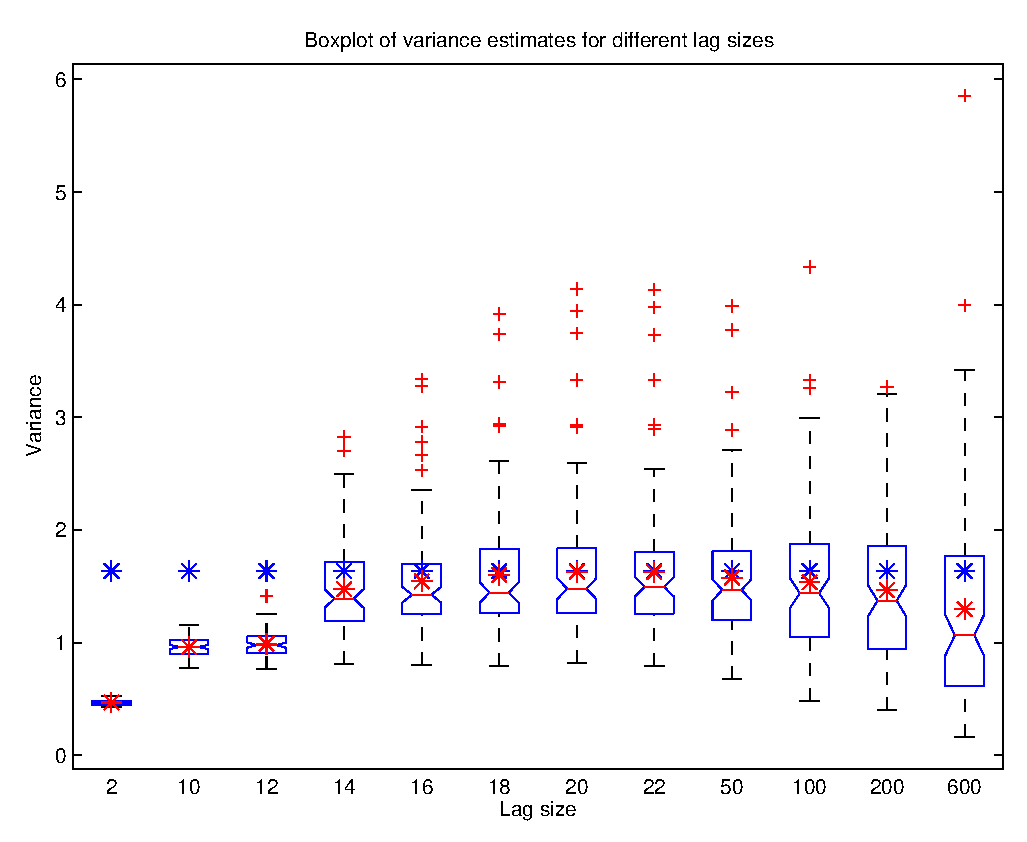
\includegraphics[width=0.8\textwidth]{boxplots_161211} % Data in fixed_lag_stovol_161211.mat
    %\vspace{-30mm}
    \caption{Estimated asymptotic variances of the particle predictor mean at time $600$ in the stochastic volatility model \eqref{eq:sto:vol:model}. The particle population size is $\N = 4,\!000$. The boxes are based on $100$ replicates of Algorithm~\ref{alg:fixed-lag:SMC} and correspond to the different lags $\lag \in \{2, 10, 12, 14, 16, 18, 20, 22, 50, 100, 200, 600\}$. The reference value $1.63$, which is indicated by blue-colored asterisks $(\ast)$, was obtained as the sample variance (scaled by the number of particles) of $1000$ independent replicates of the particle predictor mean at time $600$ (again, Algorithm~\ref{alg:fixed-lag:SMC} used $\N = 4000$ particles). Red-colored asterisks indicate average estimates.} \label{fig:boxplots:stovol}
\end{figure}

\begin{table}[H] \label{tab:lags:means:stds}
    \begin{center}
        \begin{tabular}{c|c|c} \toprule
            $\lambda$ & Mean & St. dev. \\ \midrule 
            $2$     & $.47$   & $.02$ \\
            $10$   & $.96$   & $.09$ \\ 
            $12$   & $.99$   & $.11$ \\
            $14$   & $1.47$�& $.40$ \\
            $16$   & $1.54$ & $.49$ \\
            $18$   & $1.60$ & $.57$ \\
            $20$   & $1.63$ & $.62$ \\
            $22$   & $1.62$ & $.61$ \\
            $50$   & $1.58$ & $.61$ \\
            $100$ & $1.53$ & $.71$ \\
            $200$ & $1.46$ & $.71$ \\
            $600$ & $1.30$ & $.96$ \\
        \bottomrule
        %
        \end{tabular} 
    \end{center}
    \caption{Means and standard deviations of the variance estimates reported in Figure~\ref{fig:boxplots:stovol}.} 
    \label{tab:lags:means:stds:stovol}
\end{table}

\subsubsection{Long-term stability}
\label{sec:long:term:stability}

In order to investigate numerically the long-term stability of our fixed-lag estimator, we executed Algorithm~\ref{alg:fixed-lag:SMC} on a considerably longer observation record comprising $3500$ values generated by simulation. The number of particles was set to $\N = 5000$.� Guided by the outcome of the previous experiment, we furnished the estimated predictor means with variance estimates obtained in the same sweep of the data using the fixed-lag estimator with $\lag = 20$. In parallel, the CLE was computed on the same realisation of the particle cloud. Finally, the brute-force approach estimating the asymptotic variances on the basis of $1200$ replicates of the predictor mean sequence was re-applied as a reference. 

Figure~\ref{fig:variance:evolution:short} displays the time evolution of the variance estimates over the initial $200$ time steps, where only estimates corresponding to every second time step have been plotted for readability. As evident from the top panel, the CLE targets well the reference values at most time points for this relatively limited time horizon, even though slight numerical instability may be discerned towards the very end of the plot. In addition, the fixed-lag estimator closes nicely the reference values for most time points with a variance that is somewhat smaller than that of the CLE. In order to display the estimators' long-term stability properties, Figure~\ref{fig:variance:evolution:long} provides the analogous plot for the full observation record comprising $3500$ values. Again, for readability, only estimates corresponding to every $35^\mathrm{th}$ time step have been plotted. Now, as clear from the top panel, the estimates produced by the CLE degenerate rapidly and after, say, $1500$ time steps the CLE loses track completely of the reference values. From time step $2871$, all particles in the cloud share the same Eve index, and the CLE collapses to zero. On the the contrary, from the bottom panel it is evident that the estimates delivered by the fixed-lag estimator stay numerically stable and closes well the reference values at most time points. In particular, the variance peak arising as a result of extreme state process behavior at time $3395$ is captured strikingly well by the fixed-lag estimator. 

\begin{figure}[H] % data in variance_evolution_161214b.mat
%\vspace{-25mm}
\centering
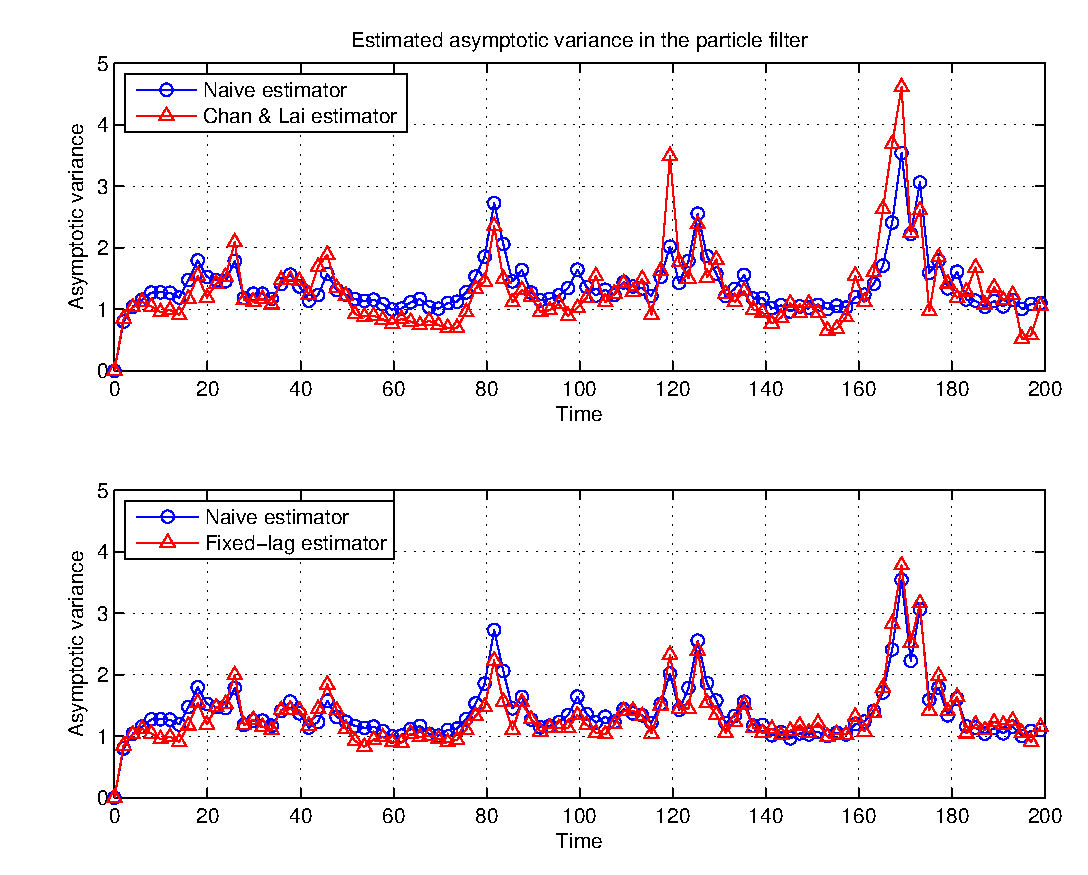
\includegraphics[width=0.8\textwidth]{variance_evolution_161214}
%\vspace{-30mm}
\caption{Long-term evolution of estimated asymptotic variances of particle predictor means in the stochastic volatility model \eqref{eq:sto:vol:model}. For clarity, only every second estimate is plotted. 
The top panel displays variance estimates ($\circ$) produced using the CLE estimator along with reference values obtained as the sample variances (scaled by the number of particles) computed from $1200$ independent replicates of the particle predictor mean sequence. The bottom panel displays the analogous plot for estimates ($\circ$) produced using the fixed-lag estimator with $\lag = 20$. The number of particles was set to $\N = 5000$ is all cases.}
 \label{fig:variance:evolution:short}
\end{figure}

\begin{figure}[H] % data in variance_evolution_161214b.mat
%\vspace{-25mm}
\centering
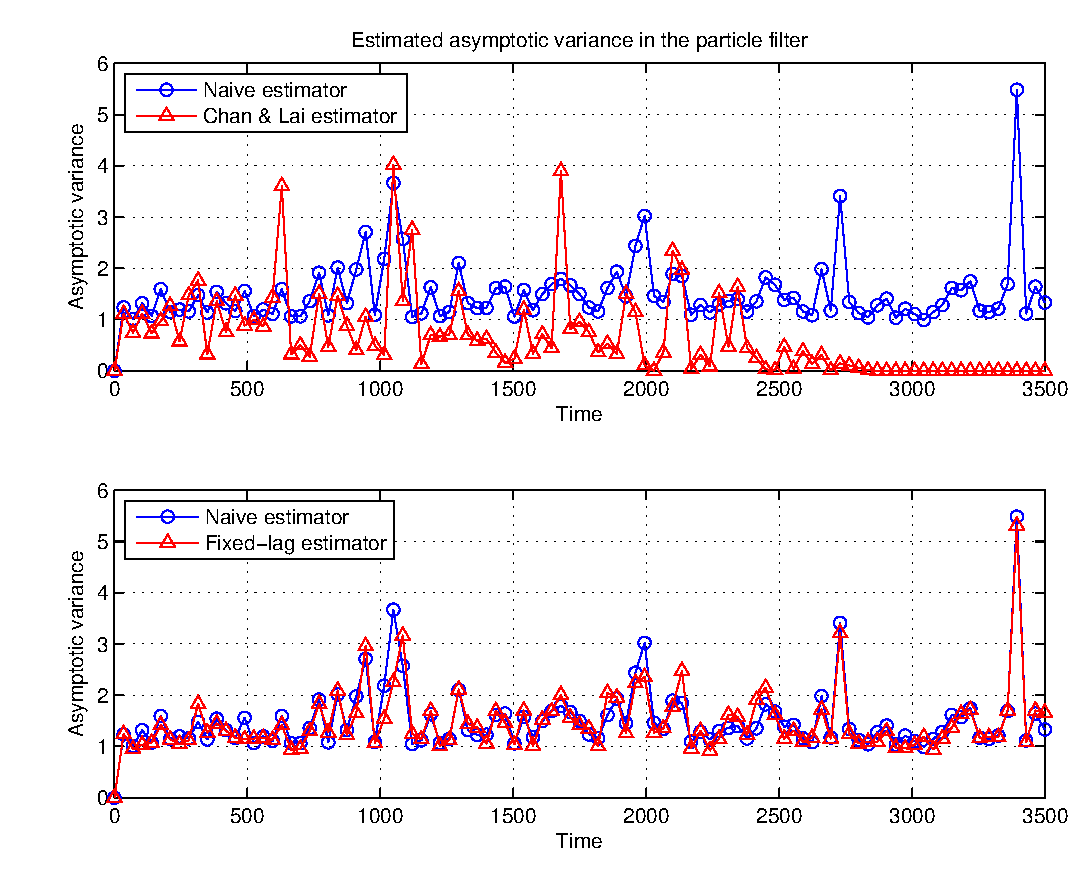
\includegraphics[width=0.8\textwidth]{variance_evolution_161214b}
%\vspace{-30mm}
\caption{The same plot as in Figure~\ref{fig:variance:evolution:short}, but now for the full observation record comprising $3500$ observations. For clarity, only every $35^{\mathrm{th}}$ estimate is plotted.}
\label{fig:variance:evolution:long}
\end{figure}



\subsection{SMC confidence bounds}
\label{sec:lin:Gauss:model}

The \emph{linear Gaussian state-space model}
\begin{equation} \label{eq:lin:Gauss:model}
\begin{split}
X_{n + 1} &= \varphi X_n + \sigma_u U_{n + 1}, \\
Y_n &= X_n + \sigma_v V_n,   
\end{split}
\quad n \in \nset, 
\end{equation}
where $\{ U_n \}_{n \in \nsetpos}$ and $\{ V_n \}_{n \in \nset}$ are again sequences of uncorrelated standard Gaussian noise, allows predictor means to be computed in a closed form using \emph{Kalman prediction} (see, e.g., \cite[Algorithm~5.2.9]{cappe:moulines:ryden:2005}). Thus, allowing comparisons with true quantities to be made, the class of linear Gaussian models is often used as a testing lab for SMC algorithms. In the setting where $|\varphi| < 1$, the state and observation processes are stationary, with zero mean Gaussian marginal stationary distributions with variances $\tilde{\sigma}^2$ and $\tilde{\sigma}^2 + \sigma_v^2$, respectively, where $\tilde{\sigma}^2 \eqdef \sigma_u^2 / (1 - \varphi^2)$. We let the former initialise the state process. 

Arguing along the lines of Section~\ref{sec:stochastic:volatility}, Assumptions~\A[assum:likelihoodDrift]{assum:majo-g} are checked straightforwardly also for this model. We leave the details to the reader.   

After having generated, for the parameterisation $(\varphi, \sigma_u, \sigma_v) = (.98, .2, 1)$, an observation record of $600$ observations, the experiment in Section~\ref{sec:lag:size:influence} was repeated for the same set of lag sizes $\lag$. As in the stochastic volatility example, the evolution of the $\N = 4000$ particles followed the same model dynamics as that generating the observations, and the reference value $1.102$ of the variance at $n = 600$ was obtained on the basis of $1000$ predictor mean replicates. The outcome is reported in Figure~\ref{fig:boxplots:lin:Gauss} and Table~\ref{tab:lags:means:stds:lin:Gauss}, which for this model indicate a somewhat even more robust performance of our estimator with respect to the lag size; indeed, more or less all the lag sizes in the interval $\intvect{12}{22}$ yield negligible biases, with only a slight increase of variance for the larger ones. According to Table~\ref{tab:lags:means:stds:lin:Gauss}, $\lambda = 18$ yields the minimal bias. As in the previous example, The CLE (corresponding to the lag size $\lambda = 600$) exhibits very unstable performance due to the relatively high $n$-to-$\N$ ratio, with at least $75\%$ of its estimates falling below the reference value. 

\begin{figure}[H] 
%\vspace{-25mm}
\centering
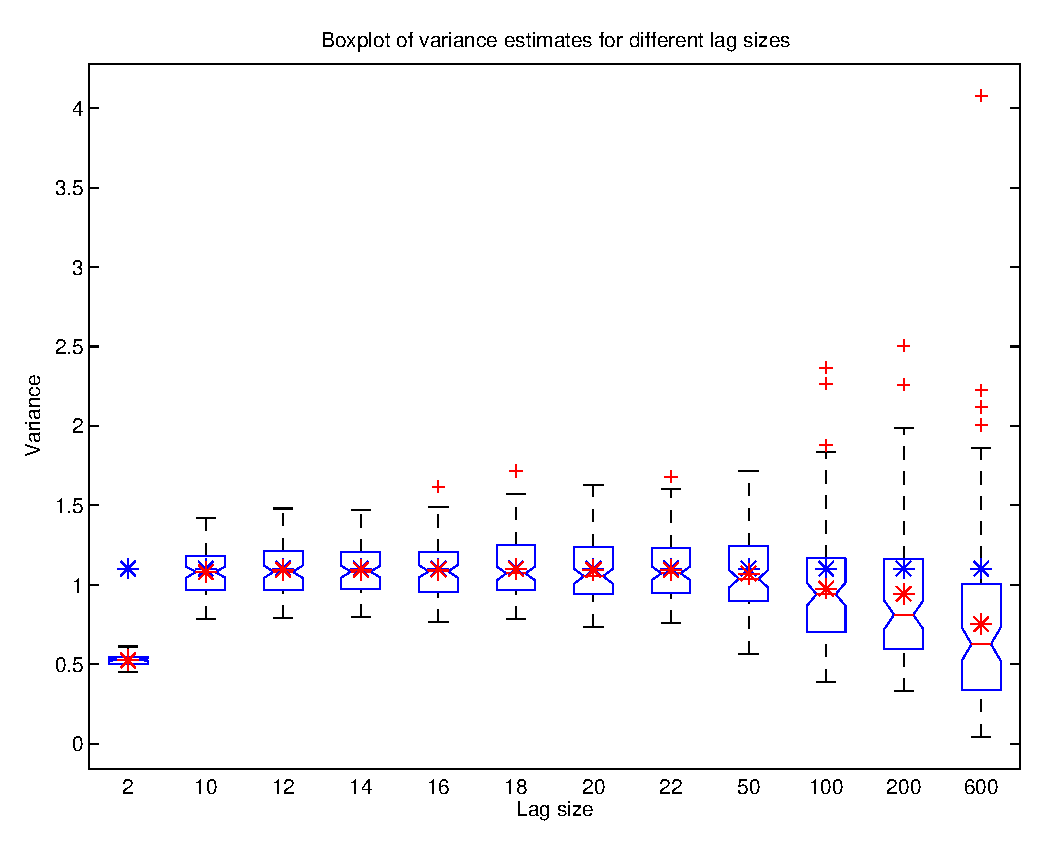
\includegraphics[width=0.8\textwidth]{boxplots_lin_Gauss_161220} % Data in fixed_lag_stovol_161220.mat
%\vspace{-30mm}
\caption{Estimated asymptotic variances of the particle predictor mean at time $600$ in the linear Gaussian model \eqref{eq:lin:Gauss:model}. The particle population size is $\N = 4000$. The boxes are based on $100$ replicates of Algorithm~\ref{alg:fixed-lag:SMC} and correspond to the different lags $\lag \in \{2, 10, 12, 14, 16, 18, 20, 22, 50, 100, 200, 600\}$. The reference value $1.102$, which is indicated by blue-colored asterisks $(\ast)$, was obtained as the sample variance (scaled by the number of particles) of $1000$ independent replicates of the particle predictor mean at time $600$ (again, Algorithm~\ref{alg:fixed-lag:SMC} used $\N = 4000$ particles). Red-colored asterisks indicate average estimates of the boxes.}
\label{fig:boxplots:lin:Gauss}
\end{figure}

\begin{table}[H] 
\begin{center}
\begin{tabular}{c|c|c} \toprule
    $\lambda$ & Mean & St. dev. \\ \midrule 
    $2$     & $.524$   & $.035$ \\
    $10$   & $1.080$ & $.157$ \\ 
    $12$   & $1.095$ & $.163$ \\
    $14$   & $1.095$�& $.162$ \\
    $16$   & $1.096$ & $.175$ \\
    $18$   & $1.099$ & $.190$ \\
    $20$   & $1.094$ & $.198$ \\
    $22$   & $1.093$ & $.202$ \\
    $50$   & $1.071$ & $.246$ \\
    $100$ & $.976$   & $.370$ \\
    $200$ & $.944$   & $.471$ \\
    $600$ & $.751$   & $.593$ \\
\bottomrule
%
\end{tabular} 
\end{center}
\caption{Means and standard deviations of the variance estimates reported in Figure~\ref{fig:boxplots:lin:Gauss}. The reference value is $1.102$} 
\label{tab:lags:means:stds:lin:Gauss}
\end{table}

Finally, using the lag $\lag = 18$ extracted from the previous simulation, Algorithm~\ref{alg:fixed-lag:SMC} was re-run $150$ times on the same observation record $\chunk{y}{0}{n - 1}$, $n = 600$, each run producing a sequence $\{ \predpart[\chunk{y}{0}{m - 1}](\operatorname{id}) \}_{m = 0}^n$ of particle predictor means, a sequence $\{ \varest{\chunk{y}{0}{m - 1}}[\lagtime{m}{\lag}](\operatorname{id}) \}_{m = 0}^n$ of fixed-lag variance estimates, and associated approximate $95\%$ confidence intervals $\{ I_m \}_{m = 0}^n$, each interval given by    
\begin{equation} \label{eq:confidence:bound}
I_m = \left(\predpart[\chunk{y}{0}{m - 1}] \operatorname{id} \pm \lambda_{.025} \frac{\varest{\chunk{y}{0}{m - 1}}[\lagtime{m}{\lag}](\operatorname{id})}{\sqrt{\N}} \right), 
\end{equation}
where $\lambda_{.025}$ denotes the $2.5\%$ quantile of the standard Gaussian distribution. As before, $\N$ was set to $4000$. In the case of effective variance estimation, one may expect each $I_m$ to fail to cover the true predicted mean $\pred[\chunk{y}{0}{m - 1}](\operatorname{id})$ with a probability close to $5\%$. Since we are in the setting of a linear Gaussian model, the exact predictor means $\{ \pred[\chunk{y}{0}{m - 1}](\operatorname{id}) \}_{m = 0}^n$ are accessible through Kalman prediction, and we are thus able to assess the failure rates of the confidence intervals at different time points. Such failure rates are reported in Figure~\ref{fig:stemplot:FRs}, and the red-dashed line indicates the perfect rate $5\%$. For readability, only every $10^{\mathrm{th}}$ time point is reported. Appealingly, it is clear that the rates fluctuate constantly around $5\%$, without any notable time dependence. This re-confirms the numeric stability of our fixed-lag variance estimator. The average failure rate across all $600$ time points was $5.5\%$. The fact that the average failure rate is slightly above the perfect rate $5\%$ is in line with the fact that the bias of our estimator is always positive, as underestimation of variance leads to more narrow confidence bounds and, consequently, higher failure rates. One way of hedging against underestimation of variance could be to replace Gaussian quantiles by the quantiles of some Student's $t$-distribution with a moderate number of degrees of freedom.  

\begin{figure}[H] 
%\vspace{-25mm}
\centering
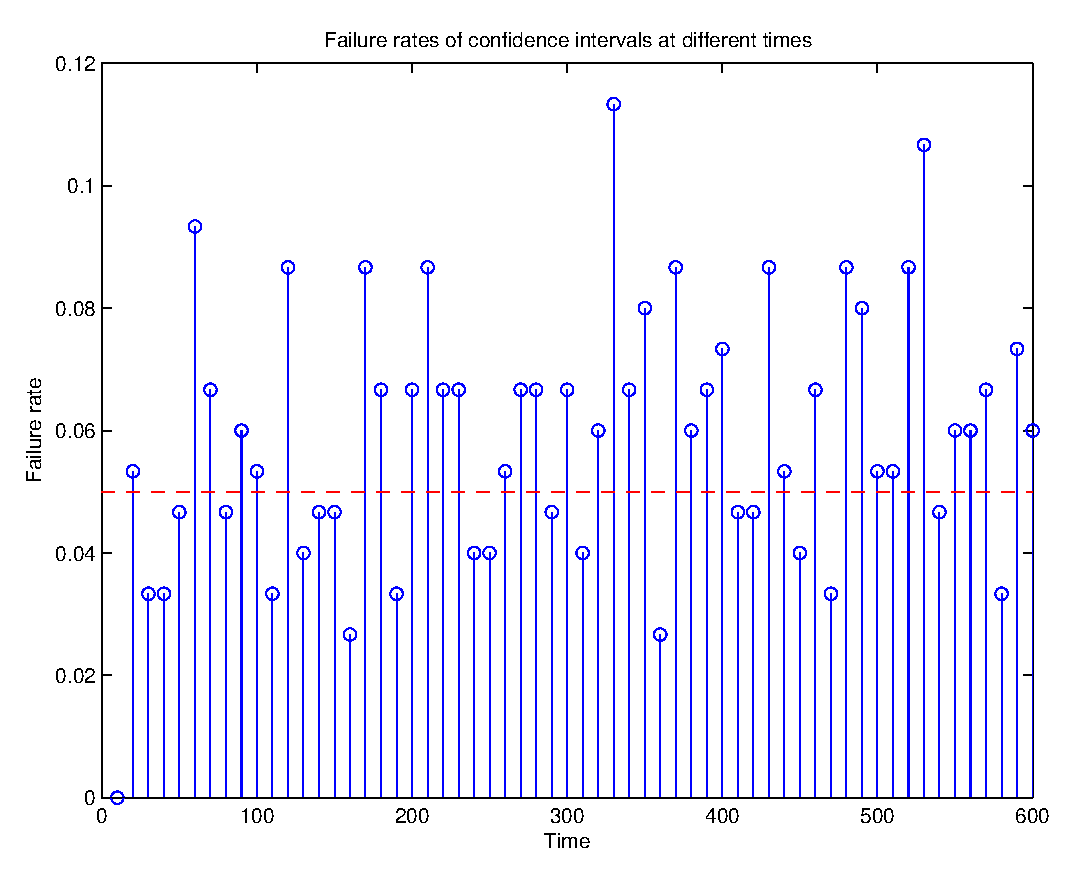
\includegraphics[width=0.8\textwidth]{stemplot_FRs} % Data in fixed_lag_lin_Gauss_161220.mat
%\vspace{-30mm}
\caption{Failure rates of confidence bounds \eqref{eq:confidence:bound} at time points $m \in \{10, 20, 30, \ldots, 600\}$. The red-dashed line indicates the perfect rate $5\%$. The failure rate estimates are based on $150$ runs of Algorithm~\ref{alg:fixed-lag:SMC} with $\N = 4000$ particles.}
\label{fig:stemplot:FRs}
\end{figure}



 

% Conclusion 
\section{Conclusion}
\label{sec:conclusion}
\section{Conclusion}
\label{sec:conclusion}

This paper presents a matrix factorization based approach to text
outlier analysis. The approach is designed to adjust well to the
widely varying structures in different localities of the data, and
therefore provides more robust methods than competing models. The
approach has the potential to be applied to other domains with
similar structure, and as a specific example, we provide experiments
on market  basket data. We also presented extensive experimental
results, which illustrate the superiority of the approach.  
Our code can be downloaded from 
\url{https://github.com/ramkikannan/outliernmf} and 
tried with any text dataset. 

In this paper, we had a parallel implementation using the
Matlab's parallel computing toolbox to run in multicore environments.
In the future, we would like to explore a scalable implementation
of our algorithm. The solution is embarrassingly parallelizable,
and would like to experiment in web scale data. One of the potential
extension is incorporating temporal and spatial aspects into the model.
Such an extension, make the solution applicable to emerging 
applications such as topic detection and streaming data. 
%In the recent times,
%approximate matrix factorization techniques are explored by
%randomly sampling the input matrix. We can reduce the computation
%time for very large matrices using such sampling techniques. We would like
%to explore a sampling based solution for our model. 
We experimented
the solution primarily on text data and market basket data. In future
work, we will extend this broader approach to other domains such as
video data.


\appendix

\section{Proofs}
\label{sec:proofs}
\subsection{Proof of Proposition~\ref{prop:consistency:fixed:lag}}
\label{sec:proof:consistency:fixed:lag}

The proof of Proposition~\ref{prop:consistency:fixed:lag} relies on the machinery developed in \cite{lee:whiteley:2016}, from which we adopt the following definitions. Throughout this section, 
let $n \in \nset$ and $\chunk{z}{0}{n - 1} \in \Zsp^n$ be picked arbitrarily.  
\begin{itemize}
\item Denote by $\Binsp{n} \eqdef \{0, 1\}^{n + 1}$ the space of binary strings of length $n + 1$. The \emph{zero string} of length $n + 1$ is denoted by $\zerostr{n}$ and for $m \in \intvect{0}{n}$, $\unitstr{m}{n}$ denotes a \emph{unit string} of length $n + 1$ with $1$ on position $m$ (with positions indexed from $0$) and zeros everywhere else.  
\item For a given string $\chunk{b}{0}{n} \in \Binsp{n}$, a Markov chain $\{�(X_m, X_m') \}_{m = 0}^n$ on $(\Xsp^2, \Xfd^{\varotimes 2})$ is defined as follows. If $b_0 = 0$, then $(X_0, X_0') \sim \init^{\varotimes 2}$; otherwise, if $b_0 = 1$, $X_0' = X_0 \sim \init$ (the initial distribution). After this, if $b_{m + 1} = 0$, $X_{m + 1} \sim \mk(X_m, \cdot)$� and $X_{m + 1}' \sim \mk(X_m', \cdot)$ conditionally independently; otherwise, if $b_{m + 1} = 1$, $X_{m + 1}' = X_{m + 1} \sim \mk(X_m, \cdot)$. 
\item With $\E_{\chunk{b}{0}{n}}$ denoting the expectation under the law of $\{�(X_m, X_m') \}_{m = 0}^n$, we define, for all $\chunk{b}{0}{n} \in \Binsp{n}$, the measures 
$$
\mu_{\chunk{b}{0}{n}} \langle \chunk{z}{0}{n - 1} \rangle : \Xfd^{\varotimes 2} \ni A \mapsto 
\E_{\chunk{b}{0}{n}} \left[ \1_A(X_n, X_n') \prod_{m = 0}^{n - 1} \pot[z_m](X_m) \pot[z_m](X_m') \right]. 
$$ 
Note that for all $h \in \bmf{\Xfd}$ it holds that $\mu_{\zerostr{n}} \langle \chunk{z}{0}{n - 1} \rangle h^{\varotimes 2} = (\init \uk[ \chunk{z}{0}{n - 1}] h)^2$ and $\mu_{\unitstr{m}{n}} \langle \chunk{z}{0}{n - 1} \rangle h^{\varotimes 2} = \init \uk[\chunk{z}{0}{m - 1}] \1_\Xsp \times \init \uk[\chunk{z}{0}{m - 1}](\uk[\chunk{z}{m}{n - 1}] h)^2$, and defining 
$$
\term[\chunk{z}{0}{n - 1}]{m}{n} : \bmf{\Xfd} \ni h \mapsto \frac{\mu_{\unitstr{m}{n}} \langle \chunk{z}{0}{n - 1} \rangle h^{\varotimes 2} - \mu_{\zerostr{n}} \langle \chunk{z}{0}{n - 1} \rangle h^{\varotimes 2}}{(\init \uk[\chunk{z}{0}{n - 1}] \1_\Xsp)^2}
$$
yields for all $h \in \bmf{\Xfd}$, 
$$
\term[\chunk{z}{0}{n - 1}]{m}{n}(h) = \frac{\pred[\chunk{z}{0}{m - 1}] (\uk[\chunk{z}{m}{n - 1}] h)^2}{(\pred[\chunk{z}{0}{m - 1}] \uk[\chunk{z}{m}{n - 1}] \1_{\Xsp})^2} - (\pred[\chunk{z}{0}{n - 1}] h)^2 
$$
and, consequently, for all $\ell \in \intvect{0}{n}$, 
\begin{equation} \label{eq:variance:alt:expression}
\variance[2]{\chunk{z}{0}{n - 1}}[\ell](h) = \sum_{m = \ell}^n \term[\chunk{z}{0}{n - 1}]{m}{n} (h - \pred[\chunk{z}{0}{n - 1}] h). 
\end{equation}
\item For all $\N \in \nsetpos$, let �$\partfd{n} \eqdef \sigma( \{ \epart{0}{i} \}_{i = 1}^\N, \{�\epart{m}{i}, \ind{m}{i} \}_{i = 1}^\N ; m \in \intvect{1}{n} )$ be the $\sigma$-field generated by the output of Algorithm~\ref{alg:SMC} during the first $n$ iterations. Conditionally on $\partfd{n}$, a genealogical trace $\chunk{\gen[1]}{0}{n}$ is formed backwards in time by, first, drawing $\gen[1]_n$ uniformly over $\intvect{1}{\N}$ and, second, setting $\gen[1]_m = \ind{m + 1}{\gen[1]_{m + 1}}$ for all $m \in \intvect{0}{n - 1}$. In addition, a parallel trace $\chunk{\gen[2]}{0}{n}$ is formed by, first, drawing $\gen[2]_n$ uniformly over $\intvect{1}{\N}$ and, second, letting $\gen[2]_m = \ind{m + 1}{\gen[2]_{m + 1}}$ if $\gen[2]_{m + 1} \neq \gen[1]_{m + 1}$ or $\gen[2]_m \sim \cat(\{ \wgt{m}{i} / \wgtsum{m} \}_{i = 1}^\N)$ otherwise. 
\end{itemize}

The proof of the following lemma follows closely that of \cite[Lemma~4]{lee:whiteley:2016} and is hence omitted. Define for all $\ell \in \intvect{0}{n}$ and $\chunk{b}{0}{\ell} \in \Binsp{\ell}$, 
$$
\binset{\ell}(\chunk{b}{0}{\ell}) \eqdef \left \{�(\chunk{k}{0}{\ell}, \chunk{k'}{0}{\ell}) \in \intvect{1}{\N}^{2(\ell + 1)} : \mbox{for all } \ell' \in \intvect{0}{\ell}, \ k_{\ell'} = k'_{\ell'} \Leftrightarrow b_{\ell'} = 1 \right \}. 
$$
\begin{lemma} \label{lemma:equiv:sets}
For all $\N \in \nsetpos$ and $m \in \intvect{0}{n}$, 
$$
\left \{ \enoch{m}{n}{\gen[1]_n} \neq \enoch{m}{n}{\gen[2]_n} \right \} = \left \{ (\chunk{\gen[1]}{m}{n}, \chunk{\gen[2]}{m}{n}) \in \binset{n - m}(0_{n - m}) \right \}. 
$$ 
\end{lemma}

In addition, define, for all $\N \in \nsetpos$, the measures
\begin{equation} \label{eq:def:part:gamma}
\unpredpart[\chunk{z}{0}{n - 1}] : \Xfd \ni A \mapsto \frac{1}{\N^{n + 1}} \left( \prod_{m = 0}^{n - 1} \wgtsum{m} \right) \sum_{i = 1}^\N \1_A(\epart{n}{i})
\end{equation}
and 
\begin{multline} \label{eq:mu:meas}
\mumeas{\N, \chunk{b}{0}{n}}{\chunk{z}{0}{n - 1}} :  \Xfd^{\varotimes 2} \ni A \mapsto 
\N^{\#_1(\chunk{b}{0}{n})} \left( \frac{\N}{\N - 1} \right)^{\#_0(\chunk{b}{0}{n})}
\left( \unpredpart[\chunk{z}{0}{n - 1}] \1_\Xsp \right)^2 \\ 
\times \E \left[ \1_A \left( \epart{n}{\gen[1]_n}, \epart{n}{\gen[2]_n} \right) \1 \left \{�(\chunk{\gen[1]}{0}{n}, \chunk{\gen[2]}{0}{n}) \in \binset{n}(\chunk{b}{0}{n}) \right \} \mid \partfd{n} \right],  
\end{multline}
where $\#_1(\chunk{b}{0}{n}) \eqdef \sum_{m = 0}^n b_m$ and $\#_0(\chunk{b}{0}{n}) \eqdef n + 1 - \#_1(\chunk{b}{0}{n})$ denote the numbers of ones and zeros in $\chunk{b}{0}{n}$, respectively. Note that \eqref{eq:def:part:gamma} implies that for all $h \in \bmf{\Xfd}$, $\predpart[\chunk{z}{0}{n - 1}] h = \unpredpart[\chunk{z}{0}{n - 1}] h / \unpredpart[\chunk{z}{0}{n - 1}] \1_\Xsp$. 

The following lemma, where first part is established in \cite[Theorem~2]{lee:whiteley:2016} and the last part is a standard result (see, e.g, \cite{douc:moulines:2008} for results on the weak consistency of SMC), will be instrumental. 

\begin{lemma} \label{lemma:mu:convergence}
For all $\chunk{b}{0}{n} \in \Binsp{n}$ and $h \in \bmf{\Xfd^{\varotimes 2}}$, as $\N \rightarrow \infty$, 
$$
\mumeas{\N, \chunk{b}{0}{n}}{\chunk{z}{0}{n - 1}} h \plim \mumeas{\chunk{b}{0}{n}}{\chunk{z}{0}{n - 1}} h. 
$$
In addition, for all $h \in \bmf{\Xfd}$, 
$$
\unpredpart[\chunk{z}{0}{n - 1}] h \plim \init \uk[\chunk{z}{0}{n - 1}] h. 
$$
\end{lemma}

\begin{proof}[Proof of Proposition~\ref{prop:consistency:fixed:lag}]
Fix $\ell \in \intvect{0}{n}$ and define for all $\N \in \nsetpos$,
\begin{multline*}
\varphi_{\N, \ell} \langle \chunk{z}{0}{n - 1} \rangle : \Xfd^{\varotimes 2} \ni A \mapsto  \left( \unpredpart[\chunk{z}{0}{n - 1}] \1_\Xsp \right)^2 \\�
\times \E \left[ \1_A \left( \epart{n}{\gen[1]_n}, \epart{n}{\gen[2]_n} \right) \1 \left \{�(\chunk{\gen[1]}{\ell}{n}, \chunk{\gen[2]}{\ell}{n}) \in \binset{n - \ell}(0_{n - \ell}) \right \} \mid \partfd{n} \right]. 
\end{multline*}
First, note that by Lemma~\ref{lemma:equiv:sets}, since $\gen[1]_n$ and $\gen[2]_n$ are conditionally independent and uniformly distributed over $\intvect{1}{\N}$, for all $h \in \bmf{\Xfd}$,  
\begin{equation} \label{eq:estimator:alt:expression}
\begin{split} 
\frac{1}{\N^2} \sum_{i = 1}^\N \left( \sum_{j : \enoch{\ell}{n}{j} = i} h(\epart{n}{j}) \right)^2 
&= \frac{1}{\N^2} \sum_{(i, j) : \enoch{\ell}{n}{i} = \enoch{\ell}{n}{j}} h(\epart{n}{i}) h(\epart{n}{j}) \\
&= (\predpart[\chunk{z}{0}{n - 1}] h)^2 - \frac{1}{\N^2} \sum_{(i, j) : \enoch{\ell}{n}{i} \neq \enoch{\ell}{n}{j}} h(\epart{n}{i}) h(\epart{n}{j}) \\
&= (\predpart[\chunk{z}{0}{n - 1}] h)^2 - \frac{\varphi_{\N, \ell} \langle \chunk{z}{0}{n - 1} \rangle h^{\varotimes 2}}{(\unpredpart[\chunk{z}{0}{n - 1}] \1_\Xsp)^2}.  
\end{split}
\end{equation}
It is hence enough to prove that for all $\N \in \nsetpos$ and $h \in \bmf{\Xfd}$, 
\begin{multline} \label{eq:sufficient:condition}
\N \left \{ (\unpredpart[\chunk{z}{0}{n - 1}] h)^2 - \varphi_{\N, \ell} \langle \chunk{z}{0}{n - 1} \rangle h^{\varotimes 2} \right\} \\�
= %\frac{1}{\N} 
\sum_{m = \ell}^n \left( \mumeas{\N, \unitstr{m}{n}}{\chunk{z}{0}{n - 1}} h^{\varotimes 2} - \mumeas{\N, \zerostr{n}}{\chunk{z}{0}{n - 1}} h^{\varotimes 2} \right) + (n - \ell + 1) (\unpredpart[\chunk{z}{0}{n - 1}] h)^2 \\�
+ \| h \|_\infty^2 \ordo(\N^{-1}),
\end{multline}
where the $\ordo(\N^{-2})$ term does not depend on $h$; indeed, along the lines of the proof of \cite[Theorem~1]{lee:whiteley:2016}, Lemma~\ref{lemma:mu:convergence} implies that for all $\chunk{b}{0}{n} \in \Binsp{n}$, as $\N \rightarrow \infty$, 
$$
\mumeas{\N, \chunk{b}{0}{n}}{\chunk{z}{0}{n - 1}} \{�h - \predpart[\chunk{z}{0}{n - 1}] h \}^{\varotimes 2} \plim \mumeas{\chunk{b}{0}{n}}{\chunk{z}{0}{n - 1}} \{�h - \pred[\chunk{z}{0}{n - 1}] h \}^{\varotimes 2}, 
$$
and \eqref{eq:sufficient:condition} hence yields, with $\ell = \lagtime{n}{\lag}$ �and when combined with \eqref{eq:estimator:alt:expression} and \eqref{eq:variance:alt:expression}, again as $\N \rightarrow \infty$, 
\begin{multline} \label{eq:critical:identity}
\varest[2]{\chunk{z}{0}{n - 1}}[\lag](h) \\
= \sum_{m = \lagtime{n}{\lag}}^n \frac{\mumeas{\N, \unitstr{m}{n}}{\chunk{z}{0}{n - 1}} \{�h - \predpart[\chunk{z}{0}{n - 1}] h \}^{\varotimes 2} - \mumeas{\N, 0_n}{\chunk{z}{0}{n - 1}} \{�h - \predpart[\chunk{z}{0}{n - 1}] h \}^{\varotimes 2}}{(\unpredpart[\chunk{z}{0}{n - 1}] \1_\Xsp)^2} \\
+ \| h \|_\infty^2 \ordo(\N^{-1}) \plim \variance[2]{\chunk{z}{0}{n - 1}}[\lagtime{n}{\lag}](h). 
\end{multline}
In order to establish \eqref{eq:sufficient:condition}, write, using that $\gen[1]_n$ and $\gen[2]_n$ are, given $ \partfd{n}$, conditionally independent and uniformly distributed over $\intvect{1}{\N}$,   
\begin{align} \label{eq:estimator:difference:form}
\lefteqn{(\unpredpart[\chunk{z}{0}{n - 1}] h)^2 - \varphi_{\N, \ell} \langle \chunk{z}{0}{n - 1} \rangle h^{\varotimes 2}} \nonumber \\ 
&= (\unpredpart[\chunk{z}{0}{n - 1}] \1_\Xsp)^2 \sum_{\chunk{b}{0}{n} \in \Binsp{n}} \E \left[ h\big( \epart{n}{\gen[1]_n} \big) h \big( \epart{n}{\gen[2]_n} \big) \1 \left \{�(\chunk{\gen[1]}{0}{n}, \chunk{\gen[2]}{0}{n}) \in \binset{n}(\chunk{b}{0}{n}) \right \} \mid \partfd{n} \right] \nonumber \\ 
&- (\unpredpart[\chunk{z}{0}{n - 1}] \1_\Xsp)^2 \sum_{\chunk{b}{0}{n} \in \Binsp{n} : \chunk{b}{\ell}{n} = 0_{n - \ell}} \E \left[ h\big( \epart{n}{\gen[1]_n} \big) h \big( \epart{n}{\gen[2]_n} \big) \1 \left \{�(\chunk{\gen[1]}{0}{n}, \chunk{\gen[2]}{0}{n}) \in \binset{n}(\chunk{b}{0}{n}) \right \} \mid \partfd{n} \right]
\end{align}
and note that, by definition \eqref{eq:mu:meas}, 
\begin{align} \label{eq:estimator:first:term}
\lefteqn{(\unpredpart[\chunk{z}{0}{n - 1}] \1_\Xsp)^2 \sum_{\chunk{b}{0}{n} \in \Binsp{n}} \E \left[ h \big( \epart{n}{\gen[1]_n} \big) h \big( \epart{n}{\gen[2]_n} \big) \1 \left \{�(\chunk{\gen[1]}{0}{n}, \chunk{\gen[2]}{0}{n}) \in \binset{n}(\chunk{b}{0}{n}) \right \} \mid \partfd{n} \right]} \nonumber \\�
&= \frac{1}{\N} \sum_{m = 0}^n \mumeas{\N, \unitstr{m}{n}}{\chunk{z}{0}{n - 1}} h^{\varotimes 2} + \left( 1 - \frac{1}{\N} \right)^{n + 1} \mumeas{\N, 0_n}{\chunk{z}{0}{n - 1}} h^{\varotimes 2} + \| h \|_\infty^2 \ordo(\N^{-2}) \nonumber \\
&= \frac{1}{\N} \sum_{m = 0}^n \left( \mumeas{\N, \unitstr{m}{n}}{\chunk{z}{0}{n - 1}} h^{\varotimes 2}  - \mumeas{\N, \zerostr{n}}{\chunk{z}{0}{n - 1}} h^{\varotimes 2} \right) + \mumeas{\N, 0_n}{\chunk{z}{0}{n - 1}} h^{\varotimes 2} + \| h \|_\infty^2 \ordo(\N^{-2}). 
\end{align}
Similarly, 
\begin{multline} \label{eq:estimator:second:term}
\lefteqn{(\unpredpart[\chunk{z}{0}{n - 1}] \1_\Xsp)^2 \sum_{\chunk{b}{0}{n} \in \Binsp{n} : \chunk{b}{\ell}{n} = 0_{n - \ell}} \E \left[ h\big( \epart{n}{\gen[1]_n} \big) h \big( \epart{n}{\gen[2]_n} \big) \1 \left \{�(\chunk{\gen[1]}{0}{n}, \chunk{\gen[2]}{0}{n}) \in \binset{n}(\chunk{b}{0}{n}) \right \} \mid \partfd{n} \right]} \\
= \frac{1}{\N} \sum_{m = 0}^{\ell - 1} \left( \mumeas{\N, \unitstr{m}{n}}{\chunk{z}{0}{n - 1}} h^{\varotimes 2}  - \mumeas{\N, \zerostr{n}}{\chunk{z}{0}{n - 1}} h^{\varotimes 2} \right) + \mumeas{\N, 0_n}{\chunk{z}{0}{n - 1}} h^{\varotimes 2} \\�
- \frac{n - \ell + 1}{\N} \mumeas{\N, 0_n}{\chunk{z}{0}{n - 1}} h^{\varotimes 2} + \| h \|_\infty^2 \ordo(\N^{-2}), 
\end{multline}
and combining \eqref{eq:estimator:difference:form}, \eqref{eq:estimator:first:term}, \eqref{eq:estimator:second:term}, and the fact that $\mumeas{0_n}{\chunk{z}{0}{n - 1}} h^{\varotimes 2} = (\init \uk[\chunk{z}{0}{n - 1}] h)^2$ yields \eqref{eq:sufficient:condition}. This completes the proof. 
\end{proof}

\subsection{Proof of Theorem~\ref{thm:tightness:bias}}

In the proof of Theorem~\ref{thm:tightness:bias}, the asymptotic bias is bounded using the time-shift approach taken in \cite[Theorem~10]{douc:moulines:olsson:2014}. Even though the theoretical analysis provided in \cite{douc:moulines:olsson:2014} is cast into the framework of general state-space models, it never makes use of the fact that $\pot$ is a normalised transition density. As stressed in \cite[Remark~1]{douc:moulines:olsson:2014}, it is hence directly applicable to the framework of randomly perturbed Feynman-Kac models in Section~\ref{sec:Feynman:Kac:models}. 

\begin{proof}
Pick arbitrarily $n \in \nset$, $\lag \in \nset$, $h \in \bmf{\Xfd}$, and $\init \in \mdr(D, r)$. 
By defining, for all $m \in \nset$, $\ell \in \intvect{0}{m - 1}$, $\chunk{z}{\ell}{m - 1} \in \Zsp^{m - \ell}$, and measures $(\mu, \mu') \in \probmeas{\Xfd}^2$, 
\begin{multline} \label{eq:def-Delta}
\Delta_{\mu, \mu'} \langle \chunk{z}{\ell}{m - 1} \rangle : \bmf{\Xfd}^2 \ni (h, h') \mapsto 
\mu \uk[\chunk{z}{\ell}{m - 1}] h \times \mu' \uk[\chunk{z}{\ell}{m - 1}] h'
\\ - \mu \uk[\chunk{z}{\ell}{m - 1}] h' \times \mu' \uk[\chunk{z}{\ell}{m - 1}] h, 
\end{multline}
we may, using the identity 
$$
\pred[\chunk{\per}{0}{m - 1}] \uk[\chunk{\per}{m}{n - 1}] \1_{\Xsp} = \frac{\init\uk[\chunk{\per}{0}{n - 1}] \1_{\Xsp}}{\init\uk[\chunk{\per}{0}{m - 1}] \1_{\Xsp}} = \prod_{\ell = m}^{n - 1} \frac{\init\uk[\chunk{\per}{0}{\ell}] \1_{\Xsp}}{\init\uk[\chunk{\per}{0}{\ell - 1}] \1_{\Xsp}} = \prod_{\ell = m}^{n - 1} \pred[\chunk{\per}{0}{\ell - 1}]  \pot[\per_\ell],
$$
for all $m \in \intvect{0}{n}$,
write the asymptotic bias at time $n$ as
\begin{equation} \label{bias:alternative:form}
\bias{\chunk{\per}{0}{n - 1}}{\lag}(h) 
= \sum_{m = 0}^{\lagtime{n}{\lag} - 1} \int \pred[\chunk{\per}{0}{m - 1}](\rmd x) \left( \frac{\DDelta{\delta_x,\pred[\chunk{\per}{0}{m - 1}]}{\chunk{\per}{m}{n - 1}}{h, \1_{\Xsp}}}
{[\prod_{\ell = m}^{n - 1} \pred[\chunk{\per}{0}{\ell - 1}]  \pot[\per_\ell]]^2} \right)^2. 
\end{equation}
In addition, under the assumptions of the theorem, \cite[Proposition~1]{douc:moulines:2012} provides the existence of a function $\pi: \Zsp^\infty \to \rset$ such that for all initial distributions $\init \in \mdr(D, r)$,
$$
\lim_{m \to \infty} \pred[\chunk{\per}{-m}{- 1}] \pot[\per_0] = \limitfunc{\chunk{\per}{- \infty}{0}}, \quad \prob\mbox{-a.s.}
$$
Since the perturbations $\{ \per_n \}_{n \in \zset}$ are stationary, the distribution of $\bias{\chunk{\per}{0}{n - 1}}{\lag}(h)$ coincides with that of the time-shifted bias $\bias{\chunk{\per}{-n}{- 1}}{\lag}(h)$, and a key step in the present proof is to express, via \eqref{bias:alternative:form}, the latter as 
\begin{multline*}
\bias{\chunk{\per}{-n}{- 1}}{\lag}(h) = \\�
\sum_{m = 0}^{\lagtime{n}{\lag} - 1} \int \pred[\chunk{\per}{-n}{- n + \lagtime{n}{\lag} - m - 2}](\rmd x) \left( \frac{\DDelta{\delta_x,\pred[\chunk{\per}{-n}{- n + \lagtime{n}{\lag} - m - 2}]}{\chunk{\per}{- n + \lagtime{n}{\lag} - m - 1}{-1}}{h, \1_{\Xsp}}}{[\prod_{\ell = 1}^{n - \lagtime{n}{\lag} + m + 1} \pred[\chunk{\per}{-n}{- \ell - 1}]  \pot[\per_{- \ell}]]^2 } \right)^2.  
\end{multline*}
We hence obtain the bound 
\begin{equation} \label{eq:fundamental:bias:bound}
\bias{\chunk{\per}{-n}{-1}}{\lag}(h) \leq A_n \times B_n,
\end{equation}
where
\begin{align*} 
A_n &\eqdef \left(\sup_{(k, m) \in \zset^2 : \, -n \leq k \leq m} \prod_{\ell = k}^{m - 1} \frac{\limitfunc{\chunk{\per}{-\infty}{\ell}}}{\pred[\chunk{\per}{-n}{\ell - 1}] \pot[\per_\ell]} \right)^4, \\ 
B_n &\eqdef \sum_{m = 0}^{\lagtime{n}{\lag} - 1} \left( \frac{\sup_{x \in \Xsp} |\DDelta{\delta_x, \pred[\chunk{\per}{-n}{- n + \lagtime{n}{\lag} - m - 2}]}{\chunk{\per}{- n + \lagtime{n}{\lag} - m - 1}{-1}}{h, \1_\Xsp}|}{[\prod_{\ell = 1}^{n - \lagtime{n}{\lag} + m + 1} \limitfunc{\chunk{\per}{-\infty}{- \ell}}]^2} \right)^2.
\end{align*}
To bound uniformly the sequence $\{ B_n \}_{n \in \nset}$, decompose each term according to 
\begin{multline} \label{eq:termwise:decomposition:Bn}
\frac{\sup_{x \in \Xsp} |\DDelta{\delta_x, \pred[\chunk{\per}{-n}{- n + \lagtime{n}{\lag} - m - 2}]}{\chunk{\per}{- n + \lagtime{n}{\lag} - m - 1}{-1}}{h, \1_\Xsp}|}{[\prod_{\ell = 1}^{n - \lagtime{n}{\lag} + m + 1} \limitfunc{\chunk{\per}{-\infty}{- \ell}}]^2} \\
= \left( \frac{\| \uk[\chunk{\per}{- n + \lagtime{n}{\lag} - m - 1}{-1}] \1_\Xsp \|_\infty}{\prod_{\ell = 1}^{n - \lagtime{n}{\lag} + m + 1} \limitfunc{\chunk{\per}{-\infty}{- \ell}}} \right)^2 \\
\times \frac{\sup_{x \in \Xsp} |\DDelta{\delta_x, \pred[\chunk{\per}{-n}{- n + \lagtime{n}{\lag} - m - 2}]}{\chunk{\per}{- n + \lagtime{n}{\lag} - m - 1}{-1}}{h, \1_\Xsp}|}{\| \uk[\chunk{\per}{- n + \lagtime{n}{\lag} - m - 1}{-1}] \1_\Xsp \|_\infty^2}. 
\end{multline}
We consider separately the two factors of \eqref{eq:termwise:decomposition:Bn}. First,
\begin{equation} \label{eq:first:factor:Bn:deomposition}
\left( \frac{\| \uk[\chunk{\per}{- n + \lagtime{n}{\lag} - m - 1}{-1}] \1_\Xsp \|_\infty}{\prod_{\ell = 1}^{n - \lagtime{n}{\lag} + m + 1} \limitfunc{\chunk{\per}{-\infty}{- \ell}}} \right)^2 = \exp\{�(n - \lagtime{n}{\lag} + m + 1) \varepsilon_{n - \lagtime{n}{\lag} + m + 1} \}, 
\end{equation}
with
$$
\varepsilon_k \eqdef \frac{2}{k} \left( \ln \| \uk[\chunk{\per}{-k}{-1}] \1_\Xsp \|_\infty - \sum_{\ell = 1}^k \ln  \limitfunc{\chunk{\per}{-\infty}{- \ell}} \right)
$$
being independent of $\init$ for all $k \in \nsetpos$.  
By \cite[Lemma~17]{douc:moulines:olsson:2014}, $\varepsilon_k \to 0$, $\prob$-a.s., as $k \to \infty$, which implies that \eqref{eq:first:factor:Bn:deomposition} grows at most subgeometrically fast with $m$.  In addition, by \cite[Proposition~16(iii)]{douc:moulines:olsson:2014} there exists a constant $\rho \in (0, 1)$ and a $\prob$-a.s. finite random variable $D$ such that for all $n$ and $m$, all $h \in \bmf{\Xfd}$, and all $\init \in \probmeas{\Xfd}$, $\prob$-a.s,
$$
\frac{\sup_{x \in \Xsp} |\DDelta{\delta_x, \pred[\chunk{\per}{-n}{- n + \lagtime{n}{\lag} - m - 2}]}{\chunk{\per}{- n + \lagtime{n}{\lag} - m - 1}{-1}}{h, \1_\Xsp}|}{\| \uk[\chunk{\per}{- n + \lagtime{n}{\lag} - m - 1}{-1}] \1_\Xsp \|_\infty^2} \leq D \rho^{n - \lagtime{n}{\lag} + m + 1} \| h \|_\infty. 
$$
Thus, $\prob$-a.s,
$$
B_n \leq D^2 \| h \|_\infty^2 \sum_{m = 0}^{\lagtime{n}{\lag} - 1} \rho^{2(n - \lagtime{n}{\lag} + m + 1)} \exp\{�2 (n - \lagtime{n}{\lag} + m + 1) \varepsilon_{n - \lagtime{n}{\lag} + m + 1} \}.  
$$
If $n \leq \lag$, then $\lagtime{n}{\lag} = 0$, and the bias vanishes. Thus, we assume in the following that $\lag < n$, which means that $\lagtime{n}{\lag} = n - \lag$. Then, by the Cauchy-Schwartz inequality, $\prob$-a.s,
\begin{align}
B_n &\leq D^2  \| h \|_\infty^2 \sum_{m = \lag + 1}^\infty \rho^{2m} \exp(2m \varepsilon_m) \nonumber \\
&\leq D^2 \| h \|_\infty^2 \left( \sum_{m = \lag + 1}^\infty \rho^{2 m} \right)^{1/2} \left( \sum_{m = \lag + 1}^\infty \rho^{2 m} \exp(4 m \varepsilon_m) \right)^{1/2} \nonumber \\
&\leq D^2 \| h \|_\infty^2 \rho^{\lag + 1} \left( \sum_{m = 0}^\infty \rho^{2 m} \right)^{1/2} \left( \sum_{m = 0}^\infty \rho^{2 m} \exp(4 m \varepsilon_m) \right)^{1/2} \nonumber \\ 
&= C \| h \|_\infty^2 \rho^{\lag + 1}, \label{eq:bias:cauchy:bound}
\end{align}
where random variable  
$$
C \eqdef D^2 \left( \sum_{m = 0}^\infty \rho^{2 m} \right)^{1/2} \left( \sum_{m = 0}^\infty \rho^{2 m} \exp(4 m \varepsilon_m) \right)^{1/2}
$$
is $\prob$-a.s. finite and independent of $\lag$, $h$, and $\init$. For $c \in \rset_+$, write, using \eqref{eq:fundamental:bias:bound} and  \eqref{eq:bias:cauchy:bound}, 
$$
\prob \left( \frac{\bias{\chunk{\per}{0}{n - 1}}{\lag}(h)}{\rate^{\lambda + 1} \| h \|_{\infty}^2} > c \right) = \prob \left( \frac{\bias{\chunk{\per}{-n}{- 1}}{\lag}(h)}{\rate^{\lambda + 1} \| h \|_{\infty}^2} > c \right) \leq \prob \left( A_n C > c \right),  
$$
where the probability on the right hand side is again independent of $\lag$, $h$, or $\init$. Thus, using the stationarity of $\{ A_n \}_{n \in \nset}$, 
$$
\prob \left( \frac{\bias{\chunk{\per}{0}{n - 1}}{\lag}(h)}{\rate^{\lambda + 1} \| h \|_{\infty}^2} > c \right) \leq \prob \left( A_0 > c^{1/2} \right)  + \prob \left( C > c^{1/2} \right), 
$$ 
where the right hand side does not depend on $n$. Now, the $\prob$-a.s. finiteness of $A_0$� was established as a part of the proof of \cite[Theorem~10]{douc:moulines:olsson:2014}. Consequently, as also $C$ is $\prob$-a.s. finite, there exists, for all $k \in \nsetpos$, a constant $c_k \in \rset_+$, independent of $\lag$, $h$, and $\init$, such that the probabilities $\prob( A_0 > c^{1/2}_k)$� and $\prob( C > c^{1/2}_k)$ are both bounded by $1/(2 k)$. This  completes the proof. 
\end{proof}

% Proof in the case of flows of updated measures

\subsection{Proof of Proposition~\ref{prop:consistency:fixed:lag:updated:case}} 

\begin{proof}
The proof consists mainly in combining some of the equalities in the proof of Proposition~\ref{prop:consistency:fixed:lag} with the identity     
\begin{multline} \label{eq:function:prod:identity}
\{�\pot[z_n] (h - \filtpart[\chunk{z}{0}{n}] h) \}^{\varotimes 2} = (\pot[z_n] h)^{\varotimes 2} - \{ (\pot[z_n] h) \varotimes \pot[z_n] \} \filtpart[\chunk{z}{0}{n}] h \\�
- \{ \pot[z_n] \varotimes (\pot[z_n] h) \} \filtpart[\chunk{z}{0}{n}] h + \pot[z_n]^{\varotimes 2} (\filtpart[\chunk{z}{0}{n}] h)^2. 
\end{multline}
More specifically, as it holds that 
\begin{equation} \label{eq:zero:identity}
\predpart[\chunk{z}{0}{n - 1}](\pot[z_n] \{ h - \filtpart[\chunk{z}{0}{n}] h \})= 0,
\end{equation}   
by reusing the equality in \eqref{eq:critical:identity},
\begin{multline} \label{eq:filtering:variance:numerator}
\varest[2]{\chunk{z}{0}{n - 1}}[\lambda](\pot[z_n] \{ h - \filtpart[\chunk{z}{0}{n}] h\}) = \\
\sum_{m = \lagtime{n}{\lag}}^n \frac{\mumeas{\N, \unitstr{m}{n}}{\chunk{z}{0}{n - 1}} \{�\pot[z_n] (h - \filtpart[\chunk{z}{0}{n}] h) \}^{\varotimes 2} - \mumeas{\N, 0_n}{\chunk{z}{0}{n - 1}} \{�\pot[z_n] (h - \filtpart[\chunk{z}{0}{n}] h) \}^{\varotimes 2}}{(\unpredpart[\chunk{z}{0}{n - 1}] \1_\Xsp)^2} \\
+ \| \pot[z_n] \|_\infty^2 \| h \|_\infty^2 \ordo(\N^{-1}). 
\end{multline}
Now, write, using \eqref{eq:function:prod:identity}, for all $\chunk{b}{0}{n} \in \Binsp{n}$, 
\begin{multline} \label{eq:termwise:decomposition:updated:case}
\mumeas{\N, \chunk{b}{0}{n}}{\chunk{z}{0}{n - 1}} \{�\pot[z_n] (h - \filtpart[\chunk{z}{0}{n}] h) \}^{\varotimes 2} =
\mumeas{\N, \chunk{b}{0}{n}}{\chunk{z}{0}{n - 1}} (\pot[z_n] h)^{\varotimes 2} \\
- \mumeas{\N, \chunk{b}{0}{n}}{\chunk{z}{0}{n - 1}} \{ (\pot[z_n] h) \varotimes \pot[z_n] \} \filtpart[\chunk{z}{0}{n}] h 
- \mumeas{\N, \chunk{b}{0}{n}}{\chunk{z}{0}{n - 1}} \{ \pot[z_n] \varotimes (\pot[z_n] h) \} \filtpart[\chunk{z}{0}{n}] h \\
+ \mumeas{\N, \chunk{b}{0}{n}}{\chunk{z}{0}{n - 1}} \pot[z_n]^{\varotimes 2} (\filtpart[\chunk{z}{0}{n}] h)^2. 
\end{multline}
Applying Lemma~\ref{lemma:mu:convergence} to each term of \eqref{eq:termwise:decomposition:updated:case} (note that the second part of Lemma~\ref{lemma:mu:convergence} implies the consistency of the updated particle measures, as 
\begin{equation} \label{eq:particle:filter:consistency}
\filtpart[\chunk{z}{0}{n}] h = \frac{\predpart[\chunk{z}{0}{n - 1}] (\pot[z_n] h)}{\predpart[\chunk{z}{0}{n - 1}] \pot[z_n]} \plim \frac{\init \uk[\chunk{z}{0}{n - 1}] (\pot[z_n] h)}{\init \uk[\chunk{z}{0}{n - 1}] \pot[z_n]} = \filt[\chunk{z}{0}{n}] h
\end{equation} 
when $\N$ tends to infinity, a now classical result) yields, using again \eqref{eq:function:prod:identity}, 
\begin{multline*}
\mumeas{\N, \chunk{b}{0}{n}}{\chunk{z}{0}{n - 1}} \{�\pot[z_n] (h - \filtpart[\chunk{z}{0}{n}] h) \}^{\varotimes 2} \plim 
\mumeas{\chunk{b}{0}{n}}{\chunk{z}{0}{n - 1}} (\pot[z_n] h)^{\varotimes 2} \\
- \mumeas{\chunk{b}{0}{n}}{\chunk{z}{0}{n - 1}} \{ (\pot[z_n] h) \varotimes \pot[z_n] \} \filt[\chunk{z}{0}{n}] h 
- \mumeas{\chunk{b}{0}{n}}{\chunk{z}{0}{n - 1}} \{ \pot[z_n] \varotimes (\pot[z_n] h) \} \filt[\chunk{z}{0}{n}] h \\
+ \mumeas{\chunk{b}{0}{n}}{\chunk{z}{0}{n - 1}} \pot[z_n]^{\varotimes 2} (\filt[\chunk{z}{0}{n}] h)^2
= \mumeas{\chunk{b}{0}{n}}{\chunk{z}{0}{n - 1}} \{�\pot[z_n] (h - \filt[\chunk{z}{0}{n}] h) \}^{\varotimes 2}, 
\end{multline*}
 as $\N$ tends to infinity. Now, applying the previous limit to \eqref{eq:filtering:variance:numerator} and using \eqref{eq:variance:alt:expression}, \eqref{eq:zero:identity}, and the second part of Lemma~\ref{lemma:mu:convergence} yields 
\begin{multline*}
\varestfilt[2]{\chunk{z}{0}{n}}[\lambda](h) = \frac{\varest[2]{\chunk{z}{0}{n - 1}}[\lambda](\pot[z_n] \{h - \filtpart[\chunk{z}{0}{n}] h\})}{(\predpart[\chunk{z}{0}{n - 1}] \pot[z_n])^2} \\�
\plim  \frac{\variance[2]{\chunk{z}{0}{n - 1}}[\lambda](\pot[z_n] \{ h - \filt[\chunk{z}{0}{n}] h \})}{(\pred[\chunk{z}{0}{n - 1}] \pot[z_n])^2} = \filtvariance[2]{\chunk{z}{0}{n}}[\lambda](h)
\end{multline*}
as $\N$ tends to infinity, which completes the proof. 
\end{proof}

\subsection{Proof of Theorem~\ref{thm:tightness:bias:filter}}

\begin{proof}
Pick arbitrarily $n \in \nset$, $\lag \in \nset$, and $h \in \bmf{\Xfd}$. Using the expression of $\filtvariance[2]{\chunk{\per}{0}{n}}(h)$� derived in the proof of \cite[Theorem~11]{douc:moulines:olsson:2014}, one may express the bias $\biasfilt{\chunk{\per}{0}{n}}{\lag}(h)$ as 
\begin{equation*} 
\biasfilt{\chunk{\per}{0}{n}}{\lag}(h) = \sum_{m = 0}^{\lagtime{n}{\lag} - 1} \int \pred[\chunk{\per}{0}{m - 1}](\rmd x) \left( \frac{\DDelta{\delta_x,\pred[\chunk{\per}{0}{m - 1}]}{\chunk{\per}{m}{n - 1}}{\pot[\per_n] h, \pot[\per_n]}}
{(\pred[\chunk{\per}{0}{m - 1}] \uk[\chunk{\per}{m}{n - 1}] \1_{\Xsp} )^2} \right)^2,  
\end{equation*}
where $\DDelta{\delta_x,\pred[\chunk{\per}{0}{m - 1}]}{\chunk{\per}{m}{n - 1}}{\pot[\per_n] h, \pot[\per_n]}$ is given by \eqref{eq:def-Delta}. Thus, the proof is finalised by following closely the lines of the proof of Theorem~\ref{thm:tightness:bias} and noting that the statement of \cite[Proposition~16(iii)]{douc:moulines:olsson:2014} still holds true when $h$� and $\1_\Xsp$ are replaced by $\pot[\per_n] h$ and $\pot[\per_n]$, respectively. 
\end{proof}

\subsection{Proof of Theorem~\ref{thm:strong:bias:bound}}
\label{sec:proof:strong:bias:bound}

\begin{proof}
If $n \leq \lag$, the bias vanishes by definition; we thus assume that $n > \lag$. Write, for $m \in \intvect{0}{n - \lag}$ and $x \in \Xsp$, 
\begin{multline} \label{eq:strong:bound:decomposition}
\frac{\uk[\chunk{z}{m}{n - 1}](h - \pred[\chunk{z}{0}{n - 1}] h)(x)}{\pred[\chunk{z}{0}{m - 1}] \uk[\chunk{z}{m}{n - 1}] \1_{\Xsp}} \\�
= \frac{\delta_x \uk[\chunk{z}{m}{n - 1}] \1_{\Xsp}}{\pred[\chunk{z}{0}{m - 1}] \uk[\chunk{z}{m}{n - 1}] \1_{\Xsp}} \left( \frac{\delta_x \uk[\chunk{z}{m}{n - 1}] h}{\delta_x \uk[\chunk{z}{m}{n - 1}] \1_{\Xsp}} - \frac{\pred[\chunk{z}{0}{m - 1}] \uk[\chunk{z}{m}{n - 1}] h}{\pred[\chunk{z}{0}{m - 1}] \uk[\chunk{z}{m}{n - 1}] \1_{\Xsp}} \right),   
\end{multline}
where \cite[Proposition~4.3.4]{delmoral:2004} bounds uniformly the second factor of \eqref{eq:strong:bound:decomposition} according to 
\begin{equation} \label{eq:strong:bound:second:term}
\left| \frac{\delta_x \uk[\chunk{z}{m}{n - 1}] h}{\delta_x \uk[\chunk{z}{m}{n - 1}] \1_{\Xsp}} - \frac{\pred[\chunk{z}{0}{m - 1}] \uk[\chunk{z}{m}{n - 1}] h}{\pred[\chunk{z}{0}{m - 1}] \uk[\chunk{z}{m}{n - 1}] \1_{\Xsp}} \right| \leq \varrho^{n - m} \| h \|_\infty. 
\end{equation}
To bound the first factor of \eqref{eq:strong:bound:decomposition}, note that
$$
\pred[\chunk{z}{0}{m - 1}] \uk[\chunk{z}{m}{n - 1}] \1_{\Xsp} = \filt[\chunk{z}{0}{m - 1}] \mk (\pot[z_m] \mk \uk[\chunk{z}{m + 1}{n - 1}] \1_{\Xsp}) \\
\geq \potlow \mdlow \mu \uk[\chunk{z}{m + 1}{n - 1}] \1_{\Xsp}
$$
and 
$$
\delta_x \uk[\chunk{z}{m}{n - 1}] \1_{\Xsp} = \pot[z_m](x) \mk \uk[\chunk{z}{m + 1}{n - 1}] \1_{\Xsp}(x) \leq \potup \mdup \mu \uk[\chunk{z}{m + 1}{n - 1}] \1_{\Xsp},
$$
where $(\mdlow, \mdup)$ and $(\potlow, \potup)$ are given in \B{ass:strong:mixing}(\ref{ass:strong:mixing-2}), implying that  
\begin{equation} \label{eq:strong:bound:first:term}
\frac{\delta_x \uk[\chunk{z}{m}{n - 1}] \1_{\Xsp}}{\pred[\chunk{z}{0}{m - 1}] \uk[\chunk{z}{m}{n - 1}] \1_{\Xsp}} \leq \frac{ \potup \mdup}{ \potlow \mdlow}.\end{equation}
Now, using \eqref{eq:strong:bound:second:term} and \eqref{eq:strong:bound:first:term}, proceed like  
\begin{multline*}
\bias{\chunk{z}{0}{n - 1}}{\lag}(h) = \sum_{m = 0}^{n - \lag - 1} \frac{\pred[\chunk{z}{0}{m - 1}] \{ \uk[\chunk{z}{m}{n - 1}](h - \pred[\chunk{z}{0}{n - 1}] h) \}^2 }{(\pred[\chunk{z}{0}{m - 1}] \uk[\chunk{z}{m}{n - 1}] \1_{\Xsp})^2} \\ 
\leq \| h \|_{\infty}^2 \left( \frac{ \potup \mdup}{ \potlow \mdlow} \right)^2  \sum_{m = 0}^{n - \lag - 1} \varrho^{2(n - m)} \leq c \| h \|_{\infty}^2 \varrho^{2(\lag + 1)}, 
\end{multline*}
with $c \eqdef (\potup \mdup / \potlow \mdlow)^2 / (1 - \varrho^2)$, and the proof is complete. 
\end{proof}












\bibliographystyle{plain}
\bibliography{mybibfile}


\end{document}
